\documentclass{article}
\usepackage{amsmath}
\usepackage{amssymb}
\usepackage{amsthm}
\usepackage{mathtools}

% Operators
\newcommand{\diag}{\operatorname{diag}}
\newcommand{\Hom}{\operatorname{Hom}}
\newcommand{\Rep}{\operatorname{Rep}}
\newcommand{\rank}{\operatorname{rank}}
\newcommand{\Supp}{\operatorname{Supp}}
\newcommand{\codim}{\operatorname{codim}}
\newcommand{\Ext}{\operatorname{Ext}}
\newcommand{\End}{\operatorname{End}}
\newcommand{\GL}{\operatorname{GL}}
\newcommand{\Lie}{\operatorname{Lie}}
\newcommand{\R}{\mathbb{R}}
\newcommand{\Mat}{\mathrm{Mat}}
\usepackage{graphicx}
\usepackage{geometry}
\usepackage{graphicx}
\usepackage{hyperref}
% Required packages for algorithms
\usepackage{algorithm}
\usepackage{algpseudocode}
\usepackage{subcaption}
\usepackage[normalem]{ulem}
\usepackage{comment}
\usepackage{tikz}
\usetikzlibrary{arrows.meta,positioning}
% theorem/proposition environments
\theoremstyle{definition}
\newtheorem{theorem}{Theorem}[section]
\newtheorem{proposition}[theorem]{Proposition}
\newtheorem{lemma}[theorem]{Lemma}
\newtheorem{corollary}[theorem]{Corollary}
\newtheorem{definition}[theorem]{Definition}
\newtheorem{remark}[theorem]{Remark}
\title{Geometry of the critical loci of deep linear networks}
\begin{document}
\maketitle
\begin{abstract}
    We study the critical loci of deep linear networks i.e. the set of parameters at which the gradient of the loss vanishes. The set of vanishing gradients can be described as an algebraic variety described by cyclic vanishing conditions. This allows us to study the fiber of the gradient map using cyclic quiver representation theory and stratify the critical loci into orbits parametrized by rank patterns i.e. the ranks of partial products of the deep linear networks weights. These orbits allow to better understand the geometry of the critical loci as the codimension of the largest irreducible component relates to the volume scaling around the critical loci of the deep linear network. 
\end{abstract}
\section{Introduction}


\subsection{Related works}


\subsection{Contributions}


\section{Setup and notations}
\begin{definition}
    A $L$ layers Deep Linear Network (DLN) is a function:
\begin{align*}
    f: \ & \mathbb{R}^{d_0} \times \prod_{l=0}^{L-1}\mathbb{R}^{d_l \times d_{l+1}}  \to \mathbb{R}^{d_L} \\
       & (x,W_1,...,W_L) \mapsto W_L...W_1 x
\end{align*}
The dimension $d_0$ is the dimension of the input data and the dimensions $d_l,\ 1\leq l \leq L$ are the width of the layers. A Deep Linear Network is a multi-linear function which is linear in each of the weight matrix $W_l$ and the data.
\end{definition}
\begin{definition}
    Consider the product map:
\begin{align*}
    \mu : & \prod_{l=0}^{L-1}\mathbb{R}^{d_l \times d_{l+1}} \to \mathbb{R}^{d_0\times d_L}\\
           &  W:=(W_1,...,W_L) \mapsto W_L...W_1
\end{align*}
This function $\mu$ maps the parameter space $\Omega:=\{(W_1,...,W_L) \in \prod_{l=0}^{L-1}\mathbb{R}^{d_l \times d_{l+1}}\}$ to the function space $\mathcal{F} \cong \mathbb{R}^{d_0\times d_L}$ of a Deep Neural Network. A DLN is a matrix-monomial (so non-linear) in the parameter space $\Omega$ (the space above) and linear map in the function space $\mathcal{F}$ (the space below).
\end{definition}
\begin{definition}
    Define the variety of matrices of rank $r$:
\begin{equation*}
    \Sigma^r_d := \{W\in\Omega|rk(W_L...W_1) = r\}
\end{equation*}
Consider the following group action of $GL_d=\Pi_{l=L}^0 GL_{d_l} = GL_{d_L}\times GL_{h} \times GL_{d_0}$:
\begin{equation*}
    (W_1,\dots,W_L)\mapsto (g_1W_1g_0^{-1},\; g_2W_2g_1^{-1},\;\dots,\; g_L W_L g_{L-1}^{-1})
\end{equation*}
We can also reparametrize $\Sigma^r_d$ by the following:
\begin{equation*}
    \Sigma^r_d = \{W\in \Omega, Z_l\in\mathbb{R}^{d_l-r\times d_{l+1}-r}| W_l \sim \begin{pmatrix} I_r & 0 \\
                                                      0.  & Z_l      
                                        \end{pmatrix}, Z_L...Z_1= 0\}
\end{equation*}
Note that the latter product over $Z$'s–the \textit{residuals}–can be defined by the algebraic variety:
\begin{equation*}
    \Sigma_0^{d -r} = \{Z_l\in\mathbb{R}^{d_l-r\times d_{l+1}-r}| Z_L...Z_1= 0\}
\end{equation*}
\end{definition}
\begin{definition}
Define the algebraic variety $\Gamma$ by the following cyclic conditions:
\begin{equation*}
    \Gamma_d^r =\{Z_l\in\mathbb{R}^{d_l-r\times d_{l+1}-r}\mid Z_{l-1}\cdots Z_1\,\Sigma_{YX}U_Q\,Z_L\cdots Z_{l+1} = 0\}
\end{equation*}
Define the algebraic variety $$\Gamma_{d,XY}:= \Sigma^{d-r}_0\cap\Gamma_d^r $$ also defined by a set of vanishing polynomial cyclic conditions.
\end{definition}
\begin{comment}
We can view $\Gamma$ as a space of quiver representations with relations.
Let $Q_\Gamma$ be the cyclic quiver with vertex set $\{0,\ldots,L\}$ and arrows
\[
    a_l: l-1 \to l \quad (l=1,\ldots,L),
    \qquad
    a_{0}: L\to 0,
\]
together with an additional distinguished arrow
\[
    a_{0}: L \to 0,
\]
A representation of $Q_\Gamma$ is given by vector spaces
$V_l\cong\mathbb{R}^{d_l-r}$ and linear maps $\phi_l:V_{s(a_l)}\to V_{t(a_l)}$.
We identify
\[
    \phi_l := Z_l \ (l=1,\ldots,L),
    \qquad
    \phi_{0} := \Sigma_{XY}U_Q : V_L \to V_0,
\]
(i.e. $\phi_{0}$ is specialized/fixed to the linear map $\Sigma_{XY}U_Q$).
Then $\Gamma$ is the subset of such representations satisfying the $L$ cyclic relations
\[
    \phi_{l-1}\cdots\phi_1\,\phi_{0}\,\phi_L\cdots\phi_{l+1}=0,
    \qquad l=1,\ldots,L,
\]
with the convention that an empty product is the identity.
If we include the condition that $$\phi_L...\phi_1=0$$ Then all paths of length $L$ are zero and we denote $\Gamma_d$ the set of paths representations satisfying this condition.
\end{comment}
\begin{proposition}
From the paper \cite{alchour}, we can write the set of rank $r$ critical points of a DLN as:
\begin{equation*}
    \mathcal{C}_r = \{W\in \Omega, Z_l\in\mathbb{R}^{d_l-r\times d_{l+1}-r}|W_L = [U_S, U_QZ_L],  W_l \sim \begin{pmatrix} I_r & 0 \\
                                                      0.  & Z_l      
                                        \end{pmatrix}, W_1 = [U_S^{\top}\Sigma_{YX}\Sigma_X^{-1}, Z_1 ]^{\top}, Z_l\in\Gamma_{d,XY}\}
\end{equation*}
Which suggest that studying the geometry of the critical loci amounts to studying the geometry of $\Gamma_{d,XY}$.
\end{proposition}
\section{Critical loci and vanishing cyclic conditions}
\begin{definition}[Block-rank stratum $\Omega_r$]\label{def:Omega_r}
Fix integers $0\le r\le \min_{0\le \ell\le L} d_\ell$ and let
\[
\Omega \;:=\; \prod_{\ell=1}^L \Mat_{d_\ell\times d_{\ell-1}}(\R)
\]
be the parameter space of depth-$L$ linear networks.
Let
\[
G \;:=\; \prod_{\ell=0}^L GL(d_\ell,\R)
\]
act on $\Omega$ by the standard change-of-basis (gauge) action
\begin{equation}\label{eq:gauge-action}
(g\cdot W)_\ell \;:=\; g_\ell\, W_\ell\, g_{\ell-1}^{-1},
\qquad
g=(g_0,\dots,g_L)\in G,\; W=(W_1,\dots,W_L)\in\Omega.
\end{equation}
For each $\ell$ define the residual matrix space
\[
\Mat^{(r)}_\ell \;:=\; \Mat_{(d_\ell-r)\times(d_{\ell-1}-r)}(\R),
\qquad
\mathcal Z \;:=\; \prod_{\ell=1}^L \Mat^{(r)}_\ell.
\]
Define the embedding $\iota:\mathcal Z\to\Omega$ by
\begin{equation}\label{eq:iota-embed}
\iota(Z)_\ell \;:=\;
\begin{pmatrix}
I_r & 0\\
0 & Z_\ell
\end{pmatrix}
\in \Mat_{d_\ell\times d_{\ell-1}}(\R),
\qquad Z=(Z_1,\dots,Z_L)\in\mathcal Z,
\end{equation}
where the block decomposition uses $\R^{d_{\ell-1}}\cong \R^r\oplus \R^{d_{\ell-1}-r}$ in the domain and
$\R^{d_\ell}\cong \R^r\oplus \R^{d_\ell-r}$ in the codomain.
Define the slice
\[
S_r \;:=\; \iota(\mathcal Z)\;\subset\;\Omega.
\]
Finally, define
\begin{equation}\label{eq:Omega_r-def}
\Omega_r \;:=\; G\cdot S_r \;=\; \{\, g\cdot \iota(Z)\;:\; g\in G,\; Z\in\mathcal Z\,\}.
\end{equation}
Equivalently, $W\in\Omega_r$ iff there exist $g\in G$ and $Z\in\mathcal Z$ such that
$W_\ell = g_\ell^{-1}\begin{pmatrix}I_r&0\\0&Z_\ell\end{pmatrix} g_{\ell-1}$ for all $\ell$ i.e. we have:
\begin{equation*}
    \Omega_r := \{W\in \Omega| W_l \sim \begin{pmatrix} I_r & 0 \\
                                                      0.  & Z_l      
                                        \end{pmatrix}, Z_l\in\mathbb{R}^{(d_l-r)\times(d_{l+1}-r)}\}
\end{equation*}
\end{definition}

\medskip

\begin{definition}[Stabilizer of the slice]\label{def:Hr}
Let $H_r\le G$ be the stabilizer subgroup of the slice $S_r$, i.e.
\[
H_r \;:=\; \{\,h\in G : h\cdot S_r = S_r\,\}.
\]
Then $H_r$ is the subgroup of block-diagonal elements of the form
\begin{equation}\label{eq:Hr-form}
H_r \;=\;
\left\{\;
h=(h_0,\dots,h_L)\in G \;:\;
h_\ell=
\begin{pmatrix}
A & 0\\
0 & K_\ell
\end{pmatrix},\;
A\in GL(r,\mathbb{R}),\;K_\ell\in GL(d_\ell-r,\mathbb{R})
\right\}.
\end{equation}
\end{definition}

\begin{proposition}[Associated bundle model for $\Omega_r$]\label{prop:associated-bundle}
Let $\Omega_r$ be as in Definition~8.1, and let $H_r$ be as in Definition~8.2. Define an action of $H_r$ on $G \times \mathcal{Z}$ by
\begin{equation}\tag{5}
(g, Z) \cdot h := \bigl(gh,\; h^{-1} \cdot Z\bigr),
\end{equation}
where for $h \in H_r$ written as in~(4),
\begin{equation}\tag{6}
(h^{-1} \cdot Z)_\ell := K_\ell^{-1}\, Z_\ell\, K_{\ell-1}, \qquad \ell = 1, \dots, L,
\end{equation}
(and $A$ acts trivially on $\mathcal{Z}$). Let $G \times_{H_r} \mathcal{Z}$ denote the quotient of $G \times \mathcal{Z}$ by this right action.

Define
\begin{equation}\tag{7}
\Phi \colon G \times \mathcal{Z} \to \Omega, \qquad \Phi(g, Z) := g \cdot \iota(Z),
\end{equation}
with $\iota$ as in~(2) and the $G$-action as in~(1). Then:
\begin{enumerate}
    \item $\Phi(G \times \mathcal{Z}) = \Omega_r$.
    \item $\Phi$ is $H_r$-invariant for the action~(5), hence descends to a well-defined map
    \[
        \bar\Phi \colon G \times_{H_r} \mathcal{Z} \longrightarrow \Omega_r, \qquad \bar\Phi([g, Z]) = \Phi(g, Z).
    \]
    Moreover, $\bar\Phi$ is surjective.
    \item Define the \emph{principal stabilizer locus}
    \[
        \mathcal{Z}^{\circ} := \bigl\{ Z \in \mathcal{Z} \;\big|\; \operatorname{Stab}_G(\iota(Z)) = H_r \bigr\},
    \]
    i.e.\ the set of $Z$ for which the only elements of $G$ mapping $\iota(Z)$ back into $S_r$ are the block-diagonal elements in $H_r$. Let $\Omega_r^{\circ} := \Phi(G \times \mathcal{Z}^{\circ})$. Then the restriction
    \[
        \bar\Phi \colon G \times_{H_r} \mathcal{Z}^{\circ} \xrightarrow{\;\sim\;} \Omega_r^{\circ}
    \]
    is a bijection. In particular, on the principal stabilizer locus,
    \begin{equation}\tag{8}
        \Omega_r^{\circ} \;\cong\; G \times_{H_r} \mathcal{Z}^{\circ}.
    \end{equation}
\end{enumerate}
\end{proposition}
The proof of the latter proposition can be found appendix \ref{app:loci-cyclic}.
\begin{remark}[Hidden-layer gauge variant]
If only hidden-layer changes of basis are allowed, replace $G$ by $G_h := \prod_{\ell=1}^{L-1} \mathrm{GL}(d_\ell, \mathbb{R})$ (i.e.\ fix $g_0, g_L$), and replace $H_r$ by $H_{r,h} := H_r \cap G_h$. All statements and the proof remain valid verbatim with this replacement, with $\mathcal{Z}^{\circ}$ redefined using $\operatorname{Stab}_{G_h}$ in place of $\operatorname{Stab}_G$.
\end{remark}
\section{Cyclic quiver representations}
\subsection{Critical loci as cyclic quivers}
A cyclic quiver is a quiver with at least one oriented cycle. In this paper, we will be interested in a quiver which is exactly one cycle here noted $C_n$.
\begin{definition}[Cyclic quiver]\label{def:cyclic-quiver}
A \emph{cyclic quiver} (or \emph{oriented cycle}) on $n\ge 1$ vertices is the quiver
$C_n$ with vertex set
\[
    P=\{0,1,\ldots,n-1\}
\]
and arrow set
\[
    E=\{a_{i}: i-1\to i\mid i=1,\ldots,n-1\}\,\cup\,\{a_{0}: n-1\to 0\},
\]
i.e. the vertices are arranged in a directed cycle.
\end{definition}

\begin{definition}[Representation of a cyclic quiver]\label{def:cyclic-quiver-representation}
A \emph{representation} of the cyclic quiver $C_n$ (arrows of $C_n$ are of the opposite orientation) over a field $k$ is the data of
vector spaces
\[
    (V_0,\ldots,V_{n-1})
\]
together with linear maps
\[
    \phi_{i}: V_{i-1}\to V_{i} \quad (i=1,\ldots,n-1),
    \qquad
    \phi_{0}: V_{n-1}\to V_{0},
\]
i.e. a representation of the opposite quiver $C_n$.
\end{definition}

\begin{proposition}[The relations defining $\Gamma$ as a cyclic quiver representation]\label{rem:Gamma-cyclic-quiver}
Fix $L\ge 1$ and consider the cyclic quiver $C_{L+1}$ on vertices
\[
    \{0,1,\ldots,L\}.
\]
Let $r$ be the rank of the student DLN and:
\[
    V_l \cong \mathbb{R}^{d_l-r}, \qquad l=0,\ldots,L,
\]
and consider a representation of the opposite quiver $C_{L+1}$ given by linear maps
\[
    \phi_{l}: V_{l-1}\to V_{l} \quad (l=1,\ldots,L)\quad \text{mod L+1}
\]
where indices are understood cyclically.

For $\phi=(\phi_0,\ldots,\phi_{L})\in \mathrm{Rep}_d(C_{L+1})$, define for
$l=1,\ldots,L$ the maps\footnote{And such that the linear compositions are compatible with the cyclic quiver}:
\[
    d\mu_{l}(\phi)
    :=
    \phi_{l-1}\cdots\phi_{1}\,
    \phi_{0}\,
    \phi_{L}\cdots\phi_{l+1} \ \in\text{Hom}(V_l,V_{l-1}) \quad \text{mod L+1}
\]
The maps $d\mu_l$ correspond to the components of the differential of the product map
around the cycle. Each map corresponds to a path of length $L$ along the cycle of length $L+1$.
Define the closed subvariety
\[
\Gamma_{d,L+1}      
:=
\Big\{
\phi\in \mathrm{Rep}_d(C_{L+1})
\;\Big|\;
d\mu_l(\phi)=0
\ \text{mod } L+1,
\ \text{for all } l=0,\ldots,L
\Big\}.
\]
Identifying DLNs with their quiver representations via $\phi_l=Z_l$ for $l=0,\ldots,L$, we now \emph{specialize the closing arrow}
\[
    \phi_{0} = \sigma:= \Sigma_{XY}U_Q : V_L \to V_0.
\]
For this specialization, the algebraic variety $\Gamma$ related to the critical loci of a DLN is:
\[
    \Gamma_{d,\sigma}
    :=
    \Gamma_{d,L+1}\big|_{\sigma=\phi_{0}=\Sigma_{XY}U_Q}
\]
coincides with the space of cyclic representations satisfying the vanishing
$d\mu$ relations and with the distinguished arrow $\phi_{0}$ fixed.
\end{proposition}

\begin{figure}[t]
    \centering
    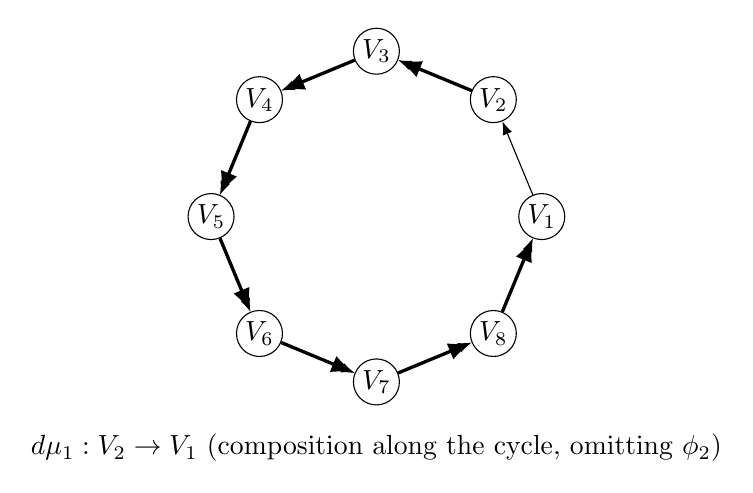
\begin{tikzpicture}[scale=1.05, every node/.style={circle,draw,inner sep=1.2pt}, >=Latex]
        % vertices on a circle
        \def\R{2.0}
        \foreach \i in {1,...,8} {
            \node (v\i) at ({\R*cos(360*(\i-1)/8)},{\R*sin(360*(\i-1)/8)}) {$V_{\i}$};
        }
        % cycle arrows
        \foreach \i [evaluate=\i as \j using {int(mod(\i,8)+1)}] in {1,...,8} {
            \draw[->] (v\i) -- (v\j);
        }
        % highlight a representative path for d\mu_l
        \draw[->,very thick] (v2) -- (v3);
        \draw[->,very thick] (v3) -- (v4);
        \draw[->,very thick] (v4) -- (v5);
        \draw[->,very thick] (v5) -- (v6);
        \draw[->,very thick] (v6) -- (v7);
        \draw[->,very thick] (v7) -- (v8);
        \draw[->,very thick] (v8) -- (v1);
        \node[draw=none,rectangle] at (0,-2.8) {$d\mu_{1}: V_2\to V_1$ (composition along the cycle, omitting $\phi_2$)};
    \end{tikzpicture}
    \caption{The cyclic quiver $C_n$ (illustrated here with $n=8$). The thick arrows indicate the path whose composition gives a typical $d\mu_l$ map along the cycle (example: $d\mu_{2}:V_2\to V_1$).}
\end{figure}

\begin{proposition}[Equivariance of the cyclic composition maps]\label{prop:mu-equivariant}
Let $C_{L+1}$ be the cyclic quiver on vertices $\{0,\ldots,L\}$, let $\mathrm{Rep}_{d}(C_{L+1})$ be its representation space with
$V_l\cong\mathbb{R}^{d_l-r}$, and let
\[\phi=(\phi_0,\ldots,\phi_L)\in \Rep_d(C_{L+1}).\]
Define the base--change group
\[
G_d:=\prod_{l=0}^{L} \mathrm{GL}(V_l)
\]
acting on $\mathrm{Rep}_{d}(C_{L+1})$ via
\[
(g\cdot \phi)_l := g_l\,\phi_l\,g_{l-1}^{-1},\quad (l=0,\ldots,L), \ \text{mod} \ L+1
\]
For each $l=1,\ldots,L$, define
\[
d\mu_l(\phi) := \phi_{l-1}\cdots\phi_1\,\phi_{0}\,\phi_L\cdots\phi_{l+1}\in\mathrm{Hom}(V_l,V_{l-1}), \quad \text{mod } L+1 
\]
with the convention that an empty product is the identity.
Then, for all $g\in G_d$ and all $l=0,\ldots,L$,
\[
d\mu_l(g\cdot \phi) = g_l\,d\mu_l(\phi)\,g_{l+1}^{-1}.
\]
\end{proposition}

\begin{proof}
Expand $d\mu_l(g\cdot\phi)$ as a product of the maps $(g\cdot\phi)_i$. Each factor contributes a left multiplication by some $g_i$ and a right multiplication by $g_{i+1}^{-1}$, and all intermediate terms cancel by associativity, leaving only $g_l$ on the left and $g_{l+1}^{-1}$ on the right.
\end{proof}

\begin{proposition}[Orbit decomposition of $\Gamma_d$]\label{prop:GammaC-orbits}
Let
\[
\Gamma_{d,L+1}:=\Big\{\phi\in \mathrm{Rep}_{d}(C_{L+1})\ \Big|\ d\mu_l(\phi)=0\ \text{for all }l=1,\ldots,L\Big\}.
\]
Then $\Gamma_{d,L+1}$ is $G_d$-invariant. In particular, $\Gamma_{d,L+1}$ decomposes as a disjoint union of $G_d$-orbits:
\[
\Gamma_{d,L+1} = \bigsqcup_{\phi\in \Gamma_{d,L+1}} G_d\cdot \phi.
\]
\end{proposition}

\begin{proof}
By Proposition~\ref{prop:mu-equivariant}, each map $d\mu_l$ is $G_d$-equivariant and hence the vanishing set $d\mu_l^{-1}(0)$ is $G_d$-stable. Intersecting over $l=1,\ldots,L$ shows that $\Gamma_{d,L+1}$ is $G_d$-stable. Any group action partitions a set into disjoint orbits, yielding the stated decomposition.
\end{proof}
Note that $\Gamma_{d,L+1}\cong \Rep_d(C_{L+1})/< d\mu_l > $, we will that $\Gamma_{d,L+1}$ is then finite dimensional and we can classify indecomposable using indecomposable representations of Nakayama algebras.
\subsection{Cyclic quiver as a bounded module}
\begin{definition}[Path algebra]
Let $Q$ be a quiver. The \emph{path algebra} $kQ$ is the $k$-vector space with basis given by all directed paths in $Q$ (including the trivial paths $e_i$ of length $0$ at each vertex $i$), with multiplication given by concatenation of composable paths and $0$ otherwise, extended by bilinearity.
\end{definition}

\begin{definition}[Bound quiver algebra associated with $\Gamma_d$]
Let $Q=C_{L+1}$ and for each $l=0,\ldots,L$ let $p_l\in kQ$ be the path
\[
 p_l := a_{l-1}\cdots a_1\,a_{0}\cdots a_{l+1},\ \text{mod } L+1
\]
interpreting empty products as the corresponding trivial path.
Let $I\subset kQ$ be the two-sided ideal generated by $\{p_0,\ldots,p_{L}\}$.
The quotient algebra
\[
A:=kQ/I
\]
is called the \emph{bound quiver algebra} associated with these relations.
\end{definition}

\begin{definition}[Representation of an algebra of dimension $d$]
Let $A$ be a $k$-algebra and let $d=(d_0,\ldots,d_L)$.
A \emph{representation of $A$ of dimension $d$ compatible with the vertices} is a left $A$-module structure on
$V:=\bigoplus_{i=0}^L k^{d_i}$ such that the idempotents $e_i\in kQ\twoheadrightarrow A$ act as the projections onto the $i$-th summand.
We denote the corresponding representation space by $\mathrm{Rep}_d(A)$.
\end{definition}

\begin{proposition}[From quiver representations with relations to $A$-modules]
There is a well-defined map
\[
F:\Gamma_{d,L+1}\to \mathrm{Rep}_d(A)
\]
which sends $\phi\in\Gamma_d$ to the unique $A$-module structure on $V$ for which each arrow $a_i$ acts by the linear map $\phi_i$.
\end{proposition}

\begin{proof}
Given $\phi\in\Gamma_{d,L+1}$, the tuple of linear maps $(\phi_i)_i$ defines a representation of the quiver $Q=C_{L+1}$, hence a left $kQ$-module structure on $V$ by letting a path act by the corresponding composition of arrow maps.
For each $l$, the defining condition $\mu_l(\phi)=0$ is exactly the statement that the element $p_l\in kQ$ acts as the zero map on $V$.
Since $I$ is the two-sided ideal generated by the $p_l$, every element of $I$ also acts by zero.
Therefore the $kQ$-action factors through the quotient $A=kQ/I$, producing a unique $A$-module structure on $V$ with the required arrow actions.
\end{proof}

\begin{proposition}[From $A$-modules to quiver representations with relations]
There is a well-defined map
\[
G:\mathrm{Rep}_d(A)\to \Gamma_{d,L+1}
\]
which sends an $A$-module structure on $V$ to the induced quiver representation $\phi$ whose arrow maps are the actions of the classes of the arrows $a_i$.
\end{proposition}

\begin{proof}
Let $V$ be a representation in $\mathrm{Rep}_d(A)$.
Composing the action map $A\to \mathrm{End}_k(V)$ with the quotient map $kQ\twoheadrightarrow A$ gives a $kQ$-module structure on $V$.
Restricting the action of each arrow basis element $a_i$ to the appropriate vertex summand yields linear maps $\phi_i:V_i\to V_{i+1}$ and hence a point $\phi\in\mathrm{Rep}_d(C_{L+1})$.
Because each $p_l$ maps to zero in $A$, it acts as the zero endomorphism on $V$.
Equivalently, the composed linear map $\mu_l(\phi)$ is zero for every $l$, so $\phi\in\Gamma_{d,L+1}$.
\end{proof}

\begin{proposition}[Correspondence between $\Gamma_{d,L+1}$ and $\mathrm{Rep}_d(A)$]
The maps $F$ and $G$ are mutually inverse bijections. In particular,
\[
\Gamma_{d,L+1} \cong \mathrm{Rep}_d(A),\qquad A=kQ/I.
\]
\end{proposition}

\begin{proof}
Starting from $\phi\in\Gamma_{d,L+1}$, the $A$-module $F(\phi)$ is by construction generated by the same arrow actions as $\phi$, so applying $G$ recovers the same tuple of arrow maps, hence $G(F(\phi))=\phi$.
Conversely, starting from an $A$-module structure on $V$, the map $G$ records the arrow actions and the map $F$ reconstructs the unique $A$-module whose arrow actions agree with those recorded, hence $F(G(V))=V$.
\end{proof}
\begin{lemma}[Finite-dimensionality of $A=kQ/I$]\label{lem:A-finite-dim}
Let $Q=C_{L+1}$ be the oriented cycle on $L+1$ vertices, and let $I\subset kQ$ be the two-sided ideal generated by the paths
$p_0,\dots,p_{L}$, where each $p_l$ is a path of length $L$ (the unique directed path going around the cycle while omitting one arrow).
Then every directed path in $Q$ of length $\ge L +1$ lies in $I$. In particular, $A=kQ/I$ is finite-dimensional.
\end{lemma}

\begin{proof}
Let $q$ be any directed path in $Q$ of length $\ge L+1$. Write $q=b_m b_{m-1}\cdots b_1$ as a concatenation of arrows with $m\ge L+1$.
Consider the contiguous subpath $q':=b_{L}\cdots b_1$ of length $L$. Since $Q$ is an oriented $L+1$-cycle, there is exactly one directed
path of length $L$ from its source to its target, hence $q'$ must coincide with one of the generators $p_l$.
Therefore $q=q''\,p_l$ for some (possibly trivial) path $q''$, so $q\in I$ because $I$ is a two-sided ideal.

Thus all paths of length $\ge L+1$ vanish in $A$, so $A$ is spanned by the residue classes of paths of length $<L+1$, a finite set. Hence $A$ is finite-dimensional.
\end{proof}

\subsection{Bounded modules are Nakayama algebras}
\begin{definition}[$A$-module]
Let $A$ be a (not necessarily commutative) $k$-algebra.
A (left) \emph{$A$-module} is a $k$-vector space $M$ together with a $k$-bilinear map
\[
A\times M\to M,\qquad (a,m)\mapsto a\cdot m,
\]
such that for all $a,b\in A$ and $m\in M$ one has
\[
(ab)\cdot m = a\cdot (b\cdot m),\qquad 1_A\cdot m = m.
\]
A \emph{homomorphism} of $A$-modules is a $k$-linear map commuting with the $A$-action.
\end{definition}

\begin{definition}[Indecomposable module]
An $A$-module $M$ is \emph{indecomposable} if $M\neq 0$ and there do not exist nonzero submodules $M_1,M_2\subset M$ such that
\[
M \cong M_1\oplus M_2.
\]
Equivalently, $M$ is indecomposable if every idempotent endomorphism of $M$ is either $0$ or $\mathrm{id}_M$.
\end{definition}

\begin{definition}[Composition series]
Let $M$ be a finite-dimensional $A$-module.
A \emph{composition series} of $M$ is a finite chain of submodules
\[
0=M_0\subset M_1\subset \cdots \subset M_{\ell}=M
\]
such that each successive quotient $M_i/M_{i-1}$ is \emph{simple}.
The integer $\ell$ is called the \emph{length} of the series.
\end{definition}

\begin{definition}[Projective module]
An $A$-module $P$ is \emph{projective} if for every surjective $A$-module homomorphism $f:M\twoheadrightarrow N$ and every $A$-module homomorphism $g:P\to N$, there exists an $A$-module homomorphism $\tilde g:P\to M$ such that $f\circ \tilde g=g$.
Equivalently, $P$ is projective if the functor $\mathrm{Hom}_A(P,-)$ is exact.
\end{definition}

\begin{definition}[Indecomposable projective module]
A \emph{projective indecomposable} $A$-module is an $A$-module that is both projective and indecomposable.
For a finite-dimensional basic algebra $A$, every indecomposable projective module is of the form $P_i\cong Ae_i$ for a primitive idempotent $e_i\in A$, and every projective module decomposes uniquely as a direct sum of indecomposable projectives.
\end{definition}

\begin{definition}[Uniserial module]
An $A$-module $M$ is \emph{uniserial} if it admits a unique composition series. Equivalently, the set of submodules of $M$ is totally ordered by inclusion.
\end{definition}
\begin{definition}[\textbf{Nakayama algebra}]
Let $A$ be a finite-dimensional $k$-algebra. We say that $A$ is a \emph{Nakayama algebra} if every indecomposable left $A$-module is \emph{uniserial}, i.e.\ it admits a unique composition series.
Equivalently, $A$ is Nakayama if every indecomposable projective left $A$-module is uniserial (and hence every indecomposable injective is uniserial).
\end{definition}

\begin{definition}[Admissible ideal]
Let $Q$ be a finite quiver and let $kQ$ be its path algebra. Write $(kQ)_{\ge m}$ for the $k$-span of all paths of length at least $m$.
A two-sided ideal $I\subset kQ$ is called \emph{admissible} if there exists an integer $m\ge 2$ such that
\[
(kQ)_{\ge m}\subseteq I \subseteq (kQ)_{\ge 2}.
\]
\end{definition}

\begin{definition}[Jacobson radical]
Let $A$ be a (not necessarily commutative) ring. The \emph{Jacobson radical} $J(A)$ is the intersection of all maximal left ideals of $A$.
If $A$ is a finite-dimensional $k$-algebra, then equivalently
\[
J(A)=\bigcap_{S\ \text{simple}} \ker\big(A\to \mathrm{End}_k(S)\big),
\]
i.e.\ $J(A)$ is the largest two-sided ideal that acts by zero on every simple $A$-module.
\end{definition}

\begin{proposition}[\textbf{Bound quiver criterion for Nakayama algebras}]\label{prop:bound-quiver-nakayama}
Let $A \simeq kQ/I$ be a finite-dimensional bound quiver algebra, where $Q$ is a finite quiver and
$I\subset kQ$ is an admissible ideal.
Assume that for every vertex $i\in Q_0$ there is at most one arrow leaving $i$ and at most one arrow entering $i$.
Then $A$ is a Nakayama algebra.

Moreover, if $Q$ is connected and has exactly one arrow leaving and exactly one arrow entering each vertex, then $Q$ is an oriented cycle and $A$ is a \emph{cyclic Nakayama algebra}. If instead $Q$ is connected and has a unique source and a unique sink, then $Q$ is an oriented line and $A$ is a \emph{linear Nakayama algebra}.
\end{proposition}

\begin{proof}
Let $e_i\in kQ\twoheadrightarrow A$ be the primitive idempotent corresponding to a vertex $i\in Q_0$, and consider the indecomposable projective module $P_i := Ae_i$.
As a $k$-vector space, $P_i$ is spanned by residue classes of paths in $Q$ starting at $i$ (modulo the relations in $I$).
Because there is at most one arrow leaving each vertex, for each $\ell\ge 0$ there is \emph{at most one} directed path of length $\ell$ starting at $i$; hence $P_i$ has a basis indexed by (the surviving classes of) these paths.

Let $J\subset A$ denote the Jacobson radical. Since $A\simeq kQ/I$ with $I$ admissible, $J$ is generated (as a two-sided ideal) by the classes of arrows, and one has
\[
J^\ell P_i = J^\ell Ae_i \ \cong\ (J^\ell)e_i,
\]
which is spanned by classes of paths of length $\ge \ell$ starting at $i$.
By the previous paragraph, for each $\ell$ the quotient $J^\ell P_i/J^{\ell+1}P_i$ is either $0$ or a simple module (it is spanned by the class of the unique surviving path of length $\ell$, if it exists).
Therefore the radical filtration
\[
P_i \supset JP_i \supset J^2P_i \supset \cdots
\]
is a chain whose successive quotients are simple (or zero), i.e.\ $P_i$ is uniserial.

Thus every indecomposable projective $P_i$ is uniserial, and hence $A$ is a Nakayama algebra.

For the final statements: if $Q$ is connected and every vertex has exactly one incoming and one outgoing arrow, then the underlying directed graph is a directed cycle. If $Q$ is connected and has a unique source and sink with all other vertices having one incoming and one outgoing arrow, then the directed graph is a directed line. These correspond to cyclic and linear Nakayama algebras respectively.
\end{proof}
\subsection{Cyclic monomial Nakayama algebra with uniform Kupisch series}
Throughout this subsection, let $Q=C_{L+1}$ be the oriented $L+1$-cycle, let $kQ$ be its path algebra, and let
\[
A:=kQ/I
\]
be the bound quiver algebra from Definition~(Bound quiver algebra associated with $\Gamma_{d,L+1}$).

\begin{definition}[Monomial (path) ideal / monomial algebra]
An ideal $I\subset kQ$ is called \emph{monomial} if it is generated (as a two-sided ideal) by paths in $Q$.
A quotient $kQ/I$ with $I$ monomial is called a \emph{monomial algebra}.
\end{definition}

\begin{definition}[Kupisch series]
Let $A$ be a finite-dimensional basic algebra with primitive idempotents $e_0,\ldots,e_{L}$ and indecomposable projectives
$P_i:=Ae_i$.
The \emph{Kupisch series} of $A$ is the $L+1$-tuple
\[
(c_0,\ldots,c_{L}),\qquad c_i:=\ell(P_i),
\]
where $\ell(P_i)$ denotes the composition length of $P_i$.
\end{definition}

\begin{remark}[Loewy length]
For a finite-dimensional algebra $A$ with Jacobson radical $J=J(A)$, the \emph{Loewy length} is the smallest integer $n$ such that $J^n=0$.
\end{remark}

\begin{proposition}[Identification and Kupisch series]
With $Q=C_{L+1}$ and $I=(p_0,\ldots,p_{L})$ as above, the algebra $A=kQ/I$ is a \emph{cyclic monomial Nakayama algebra}.
Moreover its Kupisch series is uniform:
\[
(c_0,\ldots,c_{L})=(L,\ldots,L).
\]
\end{proposition}

\begin{proof}
By construction, the ideal $I$ is generated by the paths $p_0,\ldots,p_{L}$, hence $I$ is monomial and $A$ is a monomial algebra.
By Proposition~\ref{prop:bound-quiver-nakayama}, $A$ is Nakayama; since $Q=C_{L+1}$ is an oriented cycle, $A$ is in fact \emph{cyclic} Nakayama.

Fix a vertex $i$ and consider $P_i=Ae_i$.
Modulo $I$, every path in $Q$ of length $\ge L$ starting at $i$ vanishes, while for each $t=0,1,\ldots,L-1$ there is exactly one directed path of length $t$ starting at $i$.
Therefore $P_i$ has a $k$-basis given by the residue classes of these $L$ paths (length $0$ through $L-1$).

Since $J=J(A)$ is generated by the classes of arrows (as recalled in the proof of Proposition~\ref{prop:bound-quiver-nakayama}), the radical filtration
\[
P_i \supset JP_i \supset J^2P_i \supset \cdots
\]
has successive quotients $J^tP_i/J^{t+1}P_i$ one-dimensional (hence simple) for $t=0,\ldots,L-1$, and zero thereafter.
Thus $\ell(P_i)=L$ for every $i$, which gives the Kupisch series $(L,\ldots,L)$.
\end{proof}

\begin{remark}
Equivalently, $A$ can be viewed as a \emph{truncated cycle algebra}: it is the path algebra of an oriented cycle with all paths of length $\ge L$ killed.
\end{remark}
\subsection{Indecomposable representations of Nakayama algebras}
\begin{definition}[The uniserial modules $M(i,\ell)$]
Fix $Q=C_{L+1}$ with vertices $Q_0=\{0,\dots,L\}$ and arrows $a_l:l-1\to l$ for $l=0,\dots,L$ with $a_0:0\to L$.
For $i\in Q_0$ and $0\le \ell\le L$, define a representation $M(i,\ell)$ of $Q$ by
\[
M(i,\ell)_j :=
\begin{cases}
k, & j\in\{i,i+1,\dots,i+\ell-1\}\ (\mathrm{mod}\ L + 1),\\
0, & \text{otherwise},
\end{cases}
\]
and for each arrow $a_j:j-1\to j$,
\[
M(i,\ell)_{a_j} :=
\begin{cases}
\mathrm{id}_k, & \text{if both source and target are }k,\\
0, & \text{otherwise}.
\end{cases}
\]
\end{definition}

\begin{lemma}[The relations vanish on $M(i,\ell)$]\label{lem:Miell-well-defined}
Let $Q=C_{L+1}$ and, for each $l\in\{0,\dots,L\}$, let
\[
p_l := a_{l-1}\cdots a_1\, a_{0}\cdots a_{l+1}, \quad \text{mod } L+1
\]
be the oriented path of length $L$ going once around the cycle and omitting $a_l$.
Set $A:=kQ/\langle p_0,\dots,p_{L}\rangle$.
Then, for every $i\in Q_0$ and $1\le \ell\le L$, the representation $M(i,\ell)$ factors through $A$, hence defines a finite-dimensional left $A$-module.
\end{lemma}

\begin{proof}
Fix $i$ and $\ell$. Each path $p_l$ has length $L$.
Since the support of $M(i,\ell)$ contains only $\ell\le L$ consecutive vertices, the corresponding composition along $p_l$ necessarily passes through a vertex where $M(i,\ell)$ is zero.
Therefore $p_l$ acts by the zero map on $M(i,\ell)$ for every $l$, so all generators of the ideal $\langle p_0,\dots,p_{L}\rangle$ act trivially.
Hence the $kQ$-action factors through $A$.
\end{proof}

\begin{lemma}[Uniseriality of $M(i,\ell)$]\label{lem:Miell-uniserial}
For every $i\in Q_0$ and $1\le \ell\le L$, the $A$-module $M(i,\ell)$ is uniserial, and in particular indecomposable.
\end{lemma}

\begin{proof}
Any nonzero submodule $N\subseteq M(i,\ell)$ must contain the one-dimensional space at some vertex in the support.
Because all arrow maps inside the support are identities, containing a vertex forces $N$ to contain all vertices reachable along the directed arrows within the support.
Consequently, the nonzero submodules are exactly the modules
$M(i+t,\ell-t)$ for $t=0,\dots,\ell-1$ (indices taken modulo $n$), and they form a chain under inclusion.
Thus submodules are totally ordered and $M(i,\ell)$ is uniserial.
\end{proof}

\begin{lemma}[Endomorphisms of $M(i,\ell)$]\label{lem:Miell-end}
For every $i\in Q_0$ and $1\le \ell\le L$, one has $\mathrm{End}_A\big(M(i,\ell)\big)\cong k$.
\end{lemma}

\begin{proof}
Let $f\in \mathrm{End}_A(M(i,\ell))$.
On each vertex $j$ in the support, $f$ is multiplication by some scalar $\lambda_j\in k$.
For each arrow inside the support, the arrow map is $\mathrm{id}_k$, so commutativity forces $\lambda_{j+1}=\lambda_j$.
Hence all $\lambda_j$ coincide with a single scalar $\lambda$, and $f=\lambda\,\mathrm{id}$.
\end{proof}

\begin{lemma}[Projective truncations realize $M(i,\ell)$]\label{lem:Miell-as-truncation}
Let $P(i):=Ae_i$ be the indecomposable projective at vertex $i$ and let $J:=J(A)$.
Then, for every $i\in Q_0$ and $1\le \ell\le L$, there is an isomorphism of $A$-modules
\[
P(i)/J^{\ell}P(i)\ \cong\ M(i,\ell).
\]
\end{lemma}

\begin{proof}
By Proposition~\ref{prop:bound-quiver-nakayama} and the previous subsection, $A$ is a cyclic Nakayama algebra with uniform Kupisch series $(L,\ldots,L)$.
In particular, $P(i)$ is uniserial of length $L$, and $J^tP(i)$ is spanned by residue classes of paths of length $\ge t$ starting at $i$.
Thus $P(i)/J^{\ell}P(i)$ has a basis given by the residue classes of the unique paths of lengths $0,1,\dots,\ell-1$ starting at $i$.
Under the induced quiver description, this quotient has one-dimensional spaces on the vertices $i,i+1,\dots,i+\ell-1$ (mod $L+1$) and identity maps along arrows inside the support, which is exactly $M(i,\ell)$.
\end{proof}

\begin{proposition}[Indecomposable representations of the cyclic truncated Nakayama algebra]
\label{prop:indecomp-cyclic-nakayama}
Let $Q=C_{L+1}$ be the oriented cyclic quiver with arrows $a_i:i-1\to i$ for $i=0,\dots,L \text{mod} L+1 $
For each $l\in\{0,\dots,L\}$, let $p_l$ be the path of length $L$ going once around the cycle and omitting $a_l$, and set
\[
A := kQ / \langle p_0,\dots,p_{L}\rangle.
\]
Then every finite-dimensional indecomposable left $A$-module is isomorphic to a unique module $M(i,\ell)$ with $i\in Q_0$ and $1\le \ell\le L$.
Equivalently, every indecomposable $A$-module is of the form $P(i)/J^{\ell}P(i)$ for a unique pair $(i,\ell)$.
In particular, $A$ has exactly $(L+1)L$ indecomposable modules up to isomorphism.
\end{proposition}

\begin{proof}
By Lemma~\ref{lem:Miell-well-defined}, each $M(i,\ell)$ is a well-defined finite-dimensional $A$-module, and by Lemma~\ref{lem:Miell-uniserial} it is indecomposable.

Conversely, since $A$ is Nakayama (Proposition~\ref{prop:bound-quiver-nakayama}), every indecomposable $A$-module is uniserial and hence a quotient of a unique indecomposable projective $P(i)=Ae_i$.
Its composition length is some $\ell$ with $1\le \ell\le \ell(P(i))=L$, and uniseriality forces the quotient to be $P(i)/J^{\ell}P(i)$.
By Lemma~\ref{lem:Miell-as-truncation}, this module is isomorphic to $M(i,\ell)$.

Uniqueness follows because the top simple module determines $i$ and the length determines $\ell$.
Counting pairs $(i,\ell)$ with $i\in Q_0$ and $1\le \ell\le L$ gives $(L+1)L$.
\end{proof}
More details about this can be found in the following lecture notes:
\href{https://www.math.uni-bielefeld.de/~wcrawley/1920noncommalg2/NA2.pdf}{Noncommutative Algebra 2: Representations of finite-dimensional algebras} in particular theorem and corroloray section 1.6.
We have a Krull schmidt theorem for these Nakayama algebras.
\begin{proposition}[Krull--Schmidt for the cyclic truncated Nakayama algebra]\label{prop:KS-cyclic-truncated-nakayama}
Let $A=kQ/I$ be the cyclic truncated Nakayama algebra, where $Q=C_{L+1}$ is the oriented $L+1$-cycle and $I$ is the ideal generated by the length-$(L)$ paths $p_0,\dots,p_{L}$ (equivalently, all paths of length $\ge L+1$ vanish in $A$).
Let $\mathrm{mod}\text{-}A$ denote the category of finite-dimensional left $A$-modules.
Then every $M\in \mathrm{mod}\text{-}A$ admits a decomposition as a finite direct sum of indecomposable $A$-modules.
Moreover, this decomposition is unique up to reordering and isomorphism of the indecomposable summands.
Equivalently, using the explicit indecomposables $M(i,\ell)$ from Proposition~\ref{prop:indecomp-cyclic-nakayama}, there exist uniquely determined multiplicities
$m_{i,\ell}\in\mathbb{Z}_{\ge 0}$ such that
\[
M \ \cong\ \bigoplus_{i=0}^{L} \ \bigoplus_{\ell=1}^{L} \ M(i,\ell)^{\oplus m_{i,\ell}}.
\]
\end{proposition}

\begin{proof}[Proof sketch]
Since $A$ is finite-dimensional over $k$, it is left artinian (and left noetherian), hence every object of $\mathrm{mod}\text{-}A$ has finite length.
In particular, $\mathrm{mod}\text{-}A$ is a Krull--Schmidt category: every object decomposes as a finite direct sum of indecomposables, and such a decomposition is unique up to permutation and isomorphism.

Concretely, existence follows by choosing a nonzero module $M$ and repeatedly splitting off a nontrivial direct summand until all summands are indecomposable; the process terminates because $M$ has finite length.
Uniqueness follows because each indecomposable has a local endomorphism ring (for example, by Lemma~\ref{lem:Miell-end} in the explicit classification), and the classical Krull--Schmidt--Azumaya argument applies.

Finally, Proposition~\ref{prop:indecomp-cyclic-nakayama} classifies the indecomposables as the modules $M(i,\ell)$, so any Krull--Schmidt decomposition can be rewritten uniquely in the stated multiplicity form.
\end{proof}
\textbf{Note}: This enables to parameterize the orbits of $\Gamma$ with the indecomposables representations.
\begin{comment}
\paragraph{Orbits, isomorphism classes, and multiplicity patterns.}
Fix a finite-dimensional $k$-algebra $A$ and a dimension vector $d=(d_0,\dots,d_{L})$.
Recall that
\[
\mathrm{Rep}_d(A)
=\Big\{\text{left $A$-module structures on }V=\bigoplus_{i=0}^{L} k^{d_i}\text{ such that each idempotent $e_i$ acts as the projection onto }k^{d_i}\Big\}.
\]
Let
\[
G_d:=\prod_{i=0}^{L} \mathrm{GL}(k^{d_i})
\]
act on $\mathrm{Rep}_d(A)$ by \emph{change of bases at the vertices} (equivalently, by transport of structure):
for $g=(g_0,\dots,g_L)\in G_d$ and a module structure $\rho:A\to \mathrm{End}_k(V)$, define a new module
structure $g\cdot \rho$ by
\[
(g\cdot \rho)(a)\;:=\; g\,\rho(a)\,g^{-1},\qquad g:=\bigoplus_{i=1}^n g_i\in \mathrm{GL}(V).
\]
When $A\simeq kQ/I$ is presented as a bound quiver algebra, this action is equivalently given on arrow
maps by $(g\cdot \phi)_a=g_{t(a)}\,\phi_a\,g_{s(a)}^{-1}$.
Then two points $\rho,\rho'\in \mathrm{Rep}_d(A)$ lie in the same $G_d$-orbit if and only if the corresponding
$A$-modules $(V,\rho)$ and $(V,\rho')$ are isomorphic in $\mathrm{mod}\text{-}A$.
Consequently, there is a canonical bijection
\[
\big(G_d\backslash \mathrm{Rep}_d(A)\big)\ \cong\ \Big\{\text{isomorphism classes of $A$-modules $M$ with $\dim(e_iM)=d_i$ for all $i$}\Big\}.
\]

Now specialize to the cyclic truncated Nakayama algebra $A=kQ/I$ considered above.
Its indecomposable modules are the uniserials $M(i,\ell)$ with $i\in\{0,\dots,L\}$ (indices taken modulo $L+1$) and $1\le \ell\le L$
(Proposition~\ref{prop:indecomp-cyclic-nakayama}).
By the Krull--Schmidt theorem (Proposition~\ref{prop:KS-cyclic-truncated-nakayama}), every finite-dimensional
$A$-module $M$ admits a decomposition
\[
M\ \simeq\ \bigoplus_{i=0}^{L}\ \bigoplus_{\ell=1}^{L} M(i,\ell)^{\oplus m_{i,\ell}},
\qquad m_{i,\ell}\in\mathbb{Z}_{\ge 0},
\]
and this decomposition is unique up to permutation of summands.
The multiplicities $(m_{i,\ell})$ determine (and are constrained by) the dimension vector $d$ via the \emph{covering equations}
\begin{equation}\label{eq:cyclic-multiplicity-constraints}
d_k \;=\; \sum_{i=0}^{L}\ \sum_{\ell=1}^{L} m_{i,\ell}\,\mathbf{1}\!\left\{k\in\{i,i+1,\dots,i+\ell-1\}\ (\mathrm{mod}\ L+1)\right\},
\qquad k=0,\dots,L,
\end{equation}
since $M(i,\ell)$ contributes a one-dimensional space at vertex $k$ exactly when $k$ lies in its cyclic
support interval of length $\ell$ starting at $i$.
Define the set of \emph{multiplicity patterns}
\[
M_d^{+}(A)
:=\left\{(m_{i,\ell})\in \mathbb{Z}_{\ge 0}^{L(L+1)}\ \middle|\ \text{\eqref{eq:cyclic-multiplicity-constraints} holds for all }k\right\}.
\]
Then the above discussion yields a concrete parametrization of orbits:
every $G_d$-orbit in $\mathrm{Rep}_d(A)$ corresponds to a unique isomorphism class in $\mathrm{mod}\text{-}A$,
and hence to a unique multiplicity pattern $(m_{i,\ell})\in M_d^{+}(A)$ via its Krull--Schmidt decomposition.
In other words, we obtain canonical bijections
\[
G_d\backslash \mathrm{Rep}_d(A)
\ \cong\
\Big\{\text{isomorphism classes in $\mathrm{mod}\text{-}A$ with dimension vector $d$}\Big\}
\ \cong\
M_d^{+}(A),
\]
where the last map sends an $A$-module to the multiplicities of the indecomposables $M(i,\ell)$ in its Krull--Schmidt decomposition.
\end{comment}
\begin{proposition}[Orbit stratification of $\Gamma_d$ by indecomposable Nakayama modules]
\label{prop:Gamma_orbit_stratification}

Fix $L \ge 1$ and let $Q = C_{L+1}$ be the oriented cyclic quiver on vertices
$\{0,\dots,L\}$.  
Let $A := kQ/I$ be the bound quiver algebra, where $I$ is the ideal generated by the length-$L$
paths $p_0,\dots,p_{L}$ obtained by going once around the cycle and omitting one arrow.
Let $d=(d_0,\dots,d_L)$ be a dimension vector. Define
\[
\Gamma_{d, L+1} := \left\{
\phi \in \mathrm{Rep}_d(Q)
\;\middle|\;
d\mu_\ell(\phi)=0 \text{ for all } \ell=0,\dots,L, \quad \text{mod} L+1
\right\},
\]
where
\[
d\mu_\ell(\phi) := \phi_{\ell-1}\cdots \phi_1\,\phi_{0}\,\phi_L\cdots \phi_{\ell+1}.
\]

Let
\[
G_d := \prod_{i=0}^{L} \mathrm{GL}(k^{d_i})
\]
act on $\Gamma_d$ by base change at the vertices.
\medskip
Then the following hold:
\begin{enumerate}
\item
There is an identification
\[
\Gamma_d \;\cong\; \mathrm{Rep}_d(A),
\]
under which the $G_d$-action coincides with transport of structure on $A$-modules.

\item
The algebra $A$ is a finite-dimensional cyclic Nakayama algebra.  
Its indecomposable finite-dimensional left modules are, up to isomorphism, the uniserial modules
\[
M(i,\ell), \qquad i \in \{0,\dots,L\}, \quad 1 \le \ell \le L,
\]
supported on $\ell$ consecutive vertices starting at $i$ (indices taken modulo $L+1$).

\item
Every $A$-module $M$ of dimension vector $d$ admits a unique (up to permutation)
Krull--Schmidt decomposition
\[
M \;\cong\; \bigoplus_{i=0}^{L}\;\bigoplus_{\ell=1}^{L} M(i,\ell)^{\oplus m_{i,\ell}},
\]
for uniquely determined multiplicities $m_{i,\ell} \in \mathbb{Z}_{\ge 0}$ satisfying the
dimension constraints
\[
d_k \;=\;
\sum_{i=0}^{L}\sum_{\ell=1}^{L}
m_{i,\ell}\,
\mathbf{1}\!\left\{
k \in \{i,i+1,\dots,i+\ell-1\} \ (\mathrm{mod}\ L+1)
\right\},
\quad k=0,\dots,L.
\]

Denote by $\mathcal M_d^+(A)$ the finite set of all such multiplicity patterns
$m=(m_{i,\ell})$.

\item
For each $m \in \mathcal M_d^+(A)$, define the stratum
\[
\Gamma_d^{(m)}
:=
\left\{
\phi \in \Gamma_{d,L+1}
\;\middle|\;
F(\phi) \cong
\bigoplus_{i,\ell} M(i,\ell)^{\oplus m_{i,\ell}}
\right\},
\]
where $F(\phi)$ denotes the associated $A$-module.

Then $\Gamma_d^{(m)}$ is a single $G_d$-orbit.

\item
The variety $\Gamma_d$ decomposes as a disjoint union of these orbits:
\[
\Gamma_d
\;=\;
\bigsqcup_{m \in \mathcal M_d^+(A)} \Gamma_d^{(m)}
\;=\;
\bigsqcup_{m \in \mathcal M_d^+(A)} G_d \cdot \phi_m,
\]
where $\phi_m$ is any representative whose associated $A$-module has multiplicity pattern $m$.
\end{enumerate}

\noindent
In particular, the $G_d$-orbits in $\Gamma_d$ are parameterized by the
multiplicity data of indecomposable $A$-modules, i.e.\ by the set
$\mathcal M_d^+(A)$.
\end{proposition}
\section{Stratification of vanishing cyclic conditions}
While the indecomposable representation of $\Gamma$ are parameterized by the $M(i,\ell)$ from the previous modules over Nakayama algebras we are actually interested in decomposing:
\begin{equation*}
    \Gamma_{\sigma} := \left\{(\phi_1,\ldots,\phi_{L+1})\in \mathrm{Rep}_d(C_{L+1})\;\middle|\; \phi_{l-1}\cdots\phi_1\,\phi_{L+1}\,\phi_L\cdots\phi_{l+1} = 0,\; \phi_{L+1}=\sigma\right\}.
\end{equation*}
where the map $\sigma\in \mathrm{Hom}(V_L,V_0)$ is fixed (in DLN it is $\Sigma_{XY}U_Q$).
The map
\begin{equation*}
    d\mu_{l,\sigma} := \phi_{l-1}\cdots\phi_1\,\sigma\,\phi_L\cdots\phi_{l+1}
\end{equation*}
is no longer $G_d$-equivariant.

\begin{definition}[Stabilizer group of the fixed arrow]\label{def:stabilizer-sigma}
Let $\sigma\in\mathrm{Hom}(V_L,V_0)$ be fixed. Define
\[
\mathrm{Stab}(\sigma):=\{(g_0,g_L)\in \mathrm{GL}(V_0)\times \mathrm{GL}(V_L)\mid g_0\,\sigma\,g_L^{-1}=\sigma\},
\]
and the corresponding subgroup of the base--change group
\[
G_\sigma:=\{g=(g_0,\ldots,g_L)\in \prod_{l=0}^L\mathrm{GL}(V_l)\mid (g_0,g_L)\in \mathrm{Stab}(\sigma)\}.
\]
\end{definition}

\begin{proposition}[$G_\sigma$-equivariance of the cyclic composition maps]\label{prop:mu-sigma-equivariant}
Fix $\sigma\in\mathrm{Hom}(V_L,V_0)$ and consider the representation space with $\phi_{L+1}=\sigma$.
For $\phi=(\phi_1,\ldots,\phi_L,\sigma)$ and each $l=1,\ldots,L$, define
\[
d\mu_{l,\sigma}(\phi):=\phi_{l-1}\cdots \phi_1\,\sigma\,\phi_L\cdots \phi_{l+1}\in\mathrm{Hom}(V_{l+1},V_l),
\]
with the convention that an empty product is the identity.
Then, for all $g\in G_\sigma$ and all $l$,
\[
d\mu_{l,\sigma}(g\cdot \phi)= g_l\,\mu_{l,\sigma}(\phi)\,g_{l+1}^{-1}.
\]
In particular, the subset $\Gamma_\sigma:=\bigcap_{l=1}^L d\mu_{l,\sigma}^{-1}(0)$ is $G_\sigma$-invariant.
\end{proposition}

\begin{proof}
Expand $d\mu_{l,\sigma}(g\cdot\phi)$ as a product of the maps $(g\cdot\phi)_i$.
All intermediate base-change factors cancel. The only remaining factors are $g_l$ on the left and
$g_{l+1}^{-1}$ on the right. The middle arrow is $(g\cdot\phi)_{L+1}=g_1\sigma g_L^{-1}$, which equals
$\sigma$ because $g\in G_\sigma$. 
\end{proof}
For all modules in $\Gamma_\sigma$ Krull-Schmidt applies (as a category of $A$-modules where $A$ is finite dimensional). We want to parameterize the orbits of $\Gamma_\sigma$ under the action of $G_\sigma$ and study their geometry (e.g. codimension).
\begin{lemma}[Intersection of a $G_d$--orbit with a fixed--arrow fiber]
\label{lem:orbit_fiber_intersection}
Let $L\ge 2$ and let $V_0,\dots,V_L$ be finite--dimensional vector spaces over an algebraically closed field $\Bbbk$.  
Set
\[
G_d \;:=\; \prod_{i=0}^L GL(V_i).
\]
Let $\Gamma_d$ be an affine variety equipped with an algebraic action of $G_d$.  
Assume there exists a morphism
\[
F:\Gamma_d \longrightarrow \Hom(V_L,V_0)
\]
satisfying the equivariance property
\begin{equation}
\label{eq:equivariance}
F(g\cdot x) \;=\; g_0\,F(x)\,g_L^{-1}
\qquad
\text{for all } g=(g_0,\dots,g_L)\in G_d,\; x\in\Gamma_d .
\end{equation}

Fix $\sigma\in \Hom(V_L,V_0)$ and define the fiber
\[
\Gamma_\sigma \;:=\; F^{-1}(\sigma).
\]
Define the stabilizer subgroup
\[
G_\sigma \;:=\; \{ g=(g_0,\dots,g_L)\in G_d \mid g_0\,\sigma\,g_L^{-1}=\sigma \}.
\]
Let $\mathcal O\subset \Gamma_d$ be a single $G_d$--orbit.  
Then either $\mathcal O\cap\Gamma_\sigma=\varnothing$, or else for every
$x\in\mathcal O\cap\Gamma_\sigma$ one has
\[
\mathcal O\cap\Gamma_\sigma \;=\; G_\sigma\cdot x .
\]
In particular, whenever $\mathcal O\cap\Gamma_\sigma\neq\varnothing$, this
intersection consists of a single $G_\sigma$--orbit.
\end{lemma}

\begin{proof}
We proceed in several steps.

\medskip\noindent
\textbf{Step 1: $\Gamma_\sigma$ is stable under the action of $G_\sigma$.}

Let $x\in\Gamma_\sigma$, so by definition $F(x)=\sigma$.  
Let $g\in G_\sigma$. Using the equivariance property \eqref{eq:equivariance},
\[
F(g\cdot x)
\;=\;
g_1\,F(x)\,g_L^{-1}
\;=\;
g_1\,\sigma\,g_L^{-1}.
\]
Since $g\in G_\sigma$, we have $g_1\,\sigma\,g_L^{-1}=\sigma$, and hence
$F(g\cdot x)=\sigma$. Therefore $g\cdot x\in\Gamma_\sigma$.  
This shows that $\Gamma_\sigma$ is invariant under the action of $G_\sigma$ and,
in particular,
\[
G_\sigma\cdot x \subseteq \Gamma_\sigma
\qquad
\text{for all } x\in\Gamma_\sigma .
\tag{$\ast$}
\]

\medskip\noindent
\textbf{Step 2: If $x\in\mathcal O\cap\Gamma_\sigma$, then
$G_\sigma\cdot x\subseteq \mathcal O\cap\Gamma_\sigma$.}

Let $x\in\mathcal O\cap\Gamma_\sigma$.  
Since $\mathcal O$ is a $G_d$--orbit, it is stable under the action of $G_d$ and
hence under the subgroup $G_\sigma\subseteq G_d$. Thus $G_\sigma\cdot x\subseteq
\mathcal O$.  
By $(\ast)$, $G_\sigma\cdot x\subseteq \Gamma_\sigma$.  
Combining these two inclusions gives
\[
G_\sigma\cdot x \subseteq \mathcal O\cap\Gamma_\sigma .
\tag{$\ast\ast$}
\]

\medskip\noindent
\textbf{Step 3: Any two points of $\mathcal O\cap\Gamma_\sigma$ differ by the
action of $G_\sigma$.}

Assume $x,y\in\mathcal O\cap\Gamma_\sigma$.  
Because $x$ and $y$ lie in the same $G_d$--orbit $\mathcal O$, there exists
$g=(g_1,\dots,g_L)\in G_d$ such that
\[
y = g\cdot x .
\]
Applying $F$ and using \eqref{eq:equivariance}, we obtain
\[
F(y)
\;=\;
F(g\cdot x)
\;=\;
g_1\,F(x)\,g_L^{-1}.
\]
Since $x,y\in\Gamma_\sigma$, we have $F(x)=F(y)=\sigma$. Therefore
\[
\sigma = g_1\,\sigma\,g_L^{-1}.
\]
By definition of $G_\sigma$, this implies $g\in G_\sigma$. Hence
$y=g\cdot x\in G_\sigma\cdot x$, and we conclude that
\[
\mathcal O\cap\Gamma_\sigma \subseteq G_\sigma\cdot x .
\tag{$\ast\ast\ast$}
\]

\medskip\noindent
\textbf{Step 4: Conclusion.}

If $\mathcal O\cap\Gamma_\sigma=\varnothing$, there is nothing to prove.
Otherwise choose any $x\in\mathcal O\cap\Gamma_\sigma$.  
Inclusion $(\ast\ast)$ gives $G_\sigma\cdot x\subseteq \mathcal O\cap\Gamma_\sigma$,
while inclusion $(\ast\ast\ast)$ gives the reverse inclusion. Therefore
\[
\mathcal O\cap\Gamma_\sigma = G_\sigma\cdot x .
\]
This proves that whenever the intersection is not empty, it consists of a single
$G_\sigma$--orbit. The lemma follows.
\end{proof}
\begin{proposition}[Rank label for Nakayama orbits and the fiber non-emptiness criterion over $\mathbb{R}$]
\label{prop:rank_label_and_nonemptiness_real}
Fix $L\ge 2$ and finite-dimensional real vector spaces $V_1,\dots,V_L$.
Let
\[
G_d \;:=\; \prod_{i=0}^L GL(V_i)
\qquad\text{and}\qquad
W \;:=\; \Hom_{\mathbb{R}}(V_L,V_0).
\]
Let $\Gamma_d$ be a real algebraic variety equipped with an algebraic action of $G_d$.
Assume there is a morphism of real varieties
\[
F:\Gamma_d \longrightarrow W
\]
satisfying the equivariance identity
\begin{equation}
\label{eq:equivariance_F}
F\!\big((g_0,\dots,g_L)\cdot x\big)=g_0\,F(x)\,g_L^{-1}
\qquad\text{for all } (g_0,\dots,g_L)\in G_d,\; x\in \Gamma_d .
\end{equation}

\medskip
\noindent
\textbf{Definition (Orbit label and rank label).}
Assume $\Gamma_d$ admits a decomposition into $G_d$--orbits indexed by a parameter set $\Lambda$,
\[
\Gamma_d \;=\; \bigsqcup_{\lambda\in\Lambda}\, \mathcal O_\lambda,
\]
where $\mathcal O_\lambda$ denotes the $G_d$--orbit corresponding to $\lambda$ (in the applications of this paper, $\lambda$ encodes the Krull--Schmidt multiplicities of the Nakayama indecomposables).  
For each $\lambda\in\Lambda$, define the integer
\begin{equation}
\label{eq:def_r_lambda}
r(\lambda) \;:=\; \mathrm{rank}\big(F(x)\big)\quad \text{for any } x\in \mathcal O_\lambda.
\end{equation}

\medskip
\noindent
Then the following statements hold.

\begin{enumerate}
\item[(i)] The integer $r(\lambda)$ in \eqref{eq:def_r_lambda} is well-defined, i.e.\ it does not depend on the choice of $x\in \mathcal O_\lambda$.
\item[(ii)] Fix $\sigma\in W$ and define the fiber $\Gamma_\sigma:=F^{-1}(\sigma)$. Then for every $\lambda\in\Lambda$,
\begin{equation}
\label{eq:nonemptiness}
\mathcal O_\lambda\cap \Gamma_\sigma \neq \varnothing
\qquad\Longleftrightarrow\qquad
r(\lambda)=\mathrm{rank}(\sigma).
\end{equation}
\end{enumerate}
\end{proposition}

\begin{proof}
We prove (i) and (ii) in separate steps.

\medskip\noindent
\textbf{Step 1: A basic invariance identity for ranks under left--right change of bases.}
Let $A\in GL(V_0)$, $B\in GL(V_L)$, and $T\in W=\Hom_{\mathbb{R}}(V_L,V_0)$.
Consider the map $T':=A\,T\,B^{-1}\in W$.
We have $\mathrm{rank}(T')=\mathrm{rank}(T)$.

\medskip\noindent
\textbf{Step 2: Proof of (i) (well-definedness of $r(\lambda)$).}
Fix $\lambda\in\Lambda$ and choose two points $x,y\in \mathcal O_\lambda$.
By definition of orbit, there exists $g=(g_0,\dots,g_L)\in G_d$ such that
\[
y=g\cdot x.
\]
Apply $F$ to both sides and use the equivariance identity \eqref{eq:equivariance_F}:
\[
F(y)=F(g\cdot x)=g_0\,F(x)\,g_L^{-1}.
\]
Now apply Step 1 with $A=g_0$, $B=g_L$, and $T=F(x)$. This yields
\[
\mathrm{rank}(F(y))=\mathrm{rank}(g_0\,F(x)\,g_L^{-1})=\mathrm{rank}(F(x)).
\]
Thus the rank of $F(\,\cdot\,)$ is constant along $\mathcal O_\lambda$, so the integer $r(\lambda)$
defined by \eqref{eq:def_r_lambda} is independent of the choice of $x\in\mathcal O_\lambda$.
This proves (i).

\medskip\noindent
\textbf{Step 3: A real classification fact for linear maps by rank.}
Let $S,T\in W=\Hom_{\mathbb{R}}(V_L,V_1)$. We use the following statement:

\smallskip\noindent
\emph{Claim.} If $\mathrm{rank}(S)=\mathrm{rank}(T)$, then there exist $A\in GL(V_1)$ and $B\in GL(V_L)$ such that
\begin{equation}
\label{eq:rank_equivalence}
S=A\,T\,B^{-1}.
\end{equation}

\medskip\noindent
\textbf{Step 4: Proof of (ii), forward implication.}
Assume $\mathcal O_\lambda\cap \Gamma_\sigma\neq \varnothing$.
Choose $x\in \mathcal O_\lambda\cap \Gamma_\sigma$.
By definition of $\Gamma_\sigma=F^{-1}(\sigma)$ we have $F(x)=\sigma$, hence
\[
\mathrm{rank}(\sigma)=\mathrm{rank}(F(x)).
\]
By definition of $r(\lambda)$ (and Step 2), $\mathrm{rank}(F(x))=r(\lambda)$ for any $x\in\mathcal O_\lambda$.
Therefore $\mathrm{rank}(\sigma)=r(\lambda)$, proving the forward direction of \eqref{eq:nonemptiness}.

\medskip\noindent
\textbf{Step 5: Proof of (ii), reverse implication.}
Assume $r(\lambda)=\mathrm{rank}(\sigma)$.
Choose any $x_0\in\mathcal O_\lambda$.
Then, by definition of $r(\lambda)$,
\[
\mathrm{rank}(F(x_0))=r(\lambda)=\mathrm{rank}(\sigma).
\]
By the claim in Step 3 (applied to $T=F(x_0)$ and $S=\sigma$), there exist
$A\in GL(V_0)$ and $B\in GL(V_L)$ such that
\[
\sigma=A\,F(x_0)\,B^{-1}.
\]
Define $g=(g_0,\dots,g_L)\in G_d$ by setting
\[
g_0:=A,\qquad g_L:=B,\qquad g_i:=\mathrm{Id}_{V_i}\ \text{ for } i=1,\dots,L-1.
\]
Then $g\in G_d$ and, using equivariance \eqref{eq:equivariance_F},
\[
F(g\cdot x_0)=g_0\,F(x_0)\,g_L^{-1}=A\,F(x_0)\,B^{-1}=\sigma.
\]
Hence $g\cdot x_0\in \Gamma_\sigma$.
Also, since $x_0\in\mathcal O_\lambda$ and $\mathcal O_\lambda$ is a $G_d$--orbit, we have $g\cdot x_0\in\mathcal O_\lambda$.
Therefore $g\cdot x_0\in \mathcal O_\lambda\cap \Gamma_\sigma$, so $\mathcal O_\lambda\cap \Gamma_\sigma\neq\varnothing$.

Combining Steps 4 and 5 yields \eqref{eq:nonemptiness}. This completes the proof.
\end{proof}
\begin{proposition}[Rank stratification of $\Gamma_{XY}$ by Nakayama types]
\label{prop:GammaXY_orbit_decomposition}
Let $d=(d_1,\dots,d_L)$ be a dimension vector and let
\[
\Gamma_d \subset \Rep_d(C_{L+1})
\]
be the variety defined in Section~\S9.
Recall that $\Gamma_d$ admits a decomposition into $G_d$--orbits indexed by
\[
\mathcal M_d^+ \;=\; \left\{ (m_{i,\ell}) \;\middle|\; 
\sum_{i,\ell} m_{i,\ell}\,\underline{\dim} M(i,\ell)=d
\right\},
\]
where $M(i,\ell)$ are the indecomposable modules of the cyclic Nakayama algebra
and $(m_{i,\ell})$ records their multiplicities.
For $\mathbf m=(m_{i,\ell})\in\mathcal M_d^+$, denote by
$\mathcal O_{\mathbf m}\subset\Gamma_d$ the corresponding $G_d$--orbit.

Let
\[
F:\Gamma_d\longrightarrow \Hom(V_L,V_1),
\qquad
F(\phi)=\phi_{L+1},
\]
and fix a linear map $\sigma\in\Hom(V_L,V_1)$.
Define
\[
\Gamma_{XY}:=\Gamma_\sigma:=F^{-1}(\sigma),
\qquad
G_\sigma:=\{g\in G_d:\ g_1\sigma g_L^{-1}=\sigma\}.
\]

For $\mathbf m\in\mathcal M_d^+$, define the integer
\[
r(\mathbf m)\;:=\;\mathrm{rank}\big(F(\phi)\big)
\quad\text{for any }\phi\in\mathcal O_{\mathbf m}.
\]
Then:

\begin{enumerate}
\item[(i)] The integer $r(\mathbf m)$ is well-defined (independent of the choice of
$\phi\in\mathcal O_{\mathbf m}$).

\item[(ii)] For every $\mathbf m\in\mathcal M_d^+$,
\[
\mathcal O_{\mathbf m}\cap \Gamma_{XY}\neq\varnothing
\quad\Longleftrightarrow\quad
r(\mathbf m)=\mathrm{rank}(\sigma).
\]

\item[(iii)] If $\mathcal O_{\mathbf m}\cap \Gamma_{XY}\neq\varnothing$, then
\[
\mathcal O_{\mathbf m}\cap \Gamma_{XY}
\]
is a single $G_\sigma$--orbit.

\item[(iv)] Consequently, $\Gamma_{XY}$ admits the disjoint decomposition
\[
\Gamma_{XY}
\;=\;
\bigsqcup_{\mathbf m\in\mathcal M_d^+ \;:\; r(\mathbf m)=\mathrm{rank}(\sigma)}
\big(\mathcal O_{\mathbf m}\cap \Gamma_{XY}\big),
\]
and each stratum in this decomposition is a single $G_\sigma$--orbit.
\end{enumerate}
\end{proposition}
\begin{proposition}[Rank formula for the closing arrow in terms of Nakayama multiplicities]
\label{prop:rank_formula_eps}
Work over $\mathbb{R}$. Fix $L\ge 2$ and a dimension vector $d=(d_0,\dots,d_L)$.
Let $\Gamma_d\subset \Rep_d(C_{L+1})$ be the variety from the document, and recall that
$\Gamma_d$ decomposes into $G_d$--orbits indexed by $\mathcal M_d^+$, i.e.\ for each
\[
\mathbf m=(m_{i,\ell})\in \mathcal M_d^+
\]
there is a corresponding $G_d$--orbit $\mathcal O_{\mathbf m}\subset \Gamma_d$ such that
every $\phi\in \mathcal O_{\mathbf m}$ has associated Nakayama module
\[
M(\phi)\;\cong\;\bigoplus_{i,\ell} M(i,\ell)^{\oplus m_{i,\ell}}
\]
(up to isomorphism), where $M(i,\ell)$ denote the indecomposable modules of the cyclic Nakayama algebra.

Define the morphism
\[
F:\Gamma_d\to \Hom_{\mathbb{R}}(V_L,V_1),
\qquad
F(\phi)=\phi_{L+1}.
\]
For $\mathbf m\in\mathcal M_d^+$ define
\[
r(\mathbf m)\;:=\;\rank(F(\phi))\qquad\text{for any }\phi\in\mathcal O_{\mathbf m},
\]
which is well-defined by Proposition~\ref{prop:rank_label_and_nonemptiness_real}.

\medskip
\noindent
\textbf{Definition (support interval and activity indicator).}
For an indecomposable $M(i,\ell)$, define its \emph{support interval} to be the cyclic set of vertices
\[
\Supp(i,\ell)\;:=\;\{\,i,\; i+1,\; \dots,\; i+\ell-1\,\}\subset \mathbb{Z}/(L+1)\mathbb{Z},
\]
where addition is taken modulo $L$ and we identify vertices with their residue classes.
Say that $M(i,\ell)$ is \emph{$(L\to 0)$--active} if the arrow $L\to 0$ acts nontrivially on $M(i,\ell)$,
i.e.\ if the structure map
\[
M(i,\ell)(L)\longrightarrow M(i,\ell)(0)
\]
induced by the quiver arrow $L\to 0$ is nonzero.
Define the indicator
\[
\epsilon(i,\ell)\;:=\;
\begin{cases}
1, & \text{if $M(i,\ell)$ is $(L\to 0)$--active},\\
0, & \text{otherwise}.
\end{cases}
\]

Then for every $\mathbf m=(m_{i,\ell})\in \mathcal M_d^+$ one has the formula
\begin{equation}
\label{eq:rank_formula_eps}
r(\mathbf m)\;=\;\sum_{i=0}^L\sum_{\ell=1}^L\epsilon(i,\ell)\,m_{i,\ell}.
\end{equation}
\end{proposition}

\begin{proof}
Fix $\mathbf m=(m_{i,\ell})\in \mathcal M_d^+$.
Choose any $\phi\in\mathcal O_{\mathbf m}$ and write $M:=M(\phi)$ for the corresponding Nakayama module.
By definition of $\mathcal O_{\mathbf m}$, there exists an isomorphism of modules
\begin{equation}
\label{eq:KS_decomp}
M \;\cong\;\bigoplus_{i,\ell} M(i,\ell)^{\oplus m_{i,\ell}}.
\end{equation}
We will compute $\rank(\phi_{L+1})=\rank(F(\phi))$ from this decomposition.

\medskip\noindent
\textbf{Step 1: Describe the vector spaces at vertices $0$ and $L$ using \eqref{eq:KS_decomp}.}

For each vertex $j\in\{0,L\}$ the representation space is $V_j=M(j)$.
Evaluating \eqref{eq:KS_decomp} at the vertex $j$ gives an isomorphism of real vector spaces
\begin{equation}
\label{eq:vertex_decomp}
V_j
\;=\;
M(j)
\;\cong\;
\bigoplus_{i,\ell} M(i,\ell)(j)^{\oplus m_{i,\ell}}.
\end{equation}
For cyclic Nakayama indecomposables, $M(i,\ell)(j)$ is either $0$ or a $1$--dimensional real vector space
(depending on whether $j\in \Supp(i,\ell)$). Therefore each summand in \eqref{eq:vertex_decomp} is either
$0$ or $\mathbb{R}^{m_{i,\ell}}$.

\medskip\noindent
\textbf{Step 2: The closing arrow respects the direct-sum decomposition.}

The linear map $\phi_{L+1}:V_L\to V_0$ is the structure map on the quiver arrow $L\to 0$.
Because $M$ is a direct sum of submodules as in \eqref{eq:KS_decomp}, the action of every quiver arrow,
and in particular the arrow $L\to 0$, decomposes as the direct sum of its actions on each direct summand.
Concretely, after choosing identifications as in \eqref{eq:vertex_decomp} for $j=L$ and $j=0$,
the map $\phi_{L+1}$ can be written as a block-diagonal direct sum
\begin{equation}
\label{eq:block_sum}
\phi_{L+1}
\;\cong\;
\bigoplus_{i,\ell}
\big(\phi_{L+1}\big)_{i,\ell},
\end{equation}
where
\[
\big(\phi_{L+1}\big)_{i,\ell}:\;
M(i,\ell)(L)^{\oplus m_{i,\ell}}
\longrightarrow
M(i,\ell)(1)^{\oplus m_{i,\ell}}
\]
is the map induced by $L\to 1$ on the summand $M(i,\ell)^{\oplus m_{i,\ell}}$.

\medskip\noindent
\textbf{Step 3: Compute each block $\big(\phi_{L+1}\big)_{i,\ell}$.}

Fix a pair $(i,\ell)$. There are two cases.

\smallskip\noindent
\emph{Case A: $\epsilon(i,\ell)=0$.}
By definition, $\epsilon(i,\ell)=0$ means the arrow $L\to 1$ acts trivially on $M(i,\ell)$, i.e.\ the map
\[
M(i,\ell)(L)\to M(i,\ell)(1)
\]
is the zero map. Taking $m_{i,\ell}$ copies, the induced map
\[
\big(\phi_{L+1}\big)_{i,\ell}:\;
M(i,\ell)(L)^{\oplus m_{i,\ell}}
\to
M(i,\ell)(1)^{\oplus m_{i,\ell}}
\]
is also the zero map. Hence
\begin{equation}
\label{eq:rank_block_zero}
\rank\big(\big(\phi_{L+1}\big)_{i,\ell}\big)=0.
\end{equation}

\smallskip\noindent
\emph{Case B: $\epsilon(i,\ell)=1$.}
By definition, $\epsilon(i,\ell)=1$ means the arrow $L\to 1$ acts nontrivially on $M(i,\ell)$.
For Nakayama indecomposables, both spaces $M(i,\ell)(L)$ and $M(i,\ell)(1)$ are then $1$--dimensional and
the map between them is a nonzero linear map $\mathbb{R}\to \mathbb{R}$.
Choose bases of these $1$--dimensional spaces; in these bases the map is multiplication by a nonzero scalar
$a_{i,\ell}\in \mathbb{R}^\times$.
On $m_{i,\ell}$ copies, the induced map is multiplication by the same scalar on each copy; in coordinates it is
\[
a_{i,\ell}\cdot I_{m_{i,\ell}}:\ \mathbb{R}^{m_{i,\ell}}\to \mathbb{R}^{m_{i,\ell}},
\]
which is invertible because $a_{i,\ell}\neq 0$. Therefore
\begin{equation}
\label{eq:rank_block_full}
\rank\big(\big(\phi_{L+1}\big)_{i,\ell}\big)=m_{i,\ell}.
\end{equation}

\medskip\noindent
\textbf{Step 4: Sum the ranks of the blocks.}

By \eqref{eq:block_sum}, after choosing bases compatible with the decomposition,
$\phi_{L+1}$ is block diagonal with blocks $\big(\phi_{L+1}\big)_{i,\ell}$.
The rank of a block-diagonal linear map is the sum of the ranks of its diagonal blocks
(because its image is the direct sum of the images of the blocks).
Hence
\[
\rank(\phi_{L+1})
\;=\;
\sum_{i,\ell}\rank\big(\big(\phi_{L+1}\big)_{i,\ell}\big).
\]
Substituting \eqref{eq:rank_block_zero} in Case A and \eqref{eq:rank_block_full} in Case B yields
\[
\rank(\phi_{L+1})
\;=\;
\sum_{i,\ell}\epsilon(i,\ell)\,m_{i,\ell}.
\]
By definition $r(\mathbf m)=\rank(\phi_{L+1})$ for $\phi\in\mathcal O_{\mathbf m}$, so this proves
\eqref{eq:rank_formula_eps}. 
\end{proof}
\begin{corollary}[Orbit decomposition of $\Gamma_{XY}$ indexed by $\mathcal M_d^+$]
\label{cor:GammaXY_decomposition_by_Mdplus}
Work over $\mathbb{R}$ and keep the notation of Proposition~\ref{prop:GammaXY_orbit_decomposition}
and Proposition~\ref{prop:rank_formula_eps}. In particular, $\Gamma_{XY}=\Gamma_\sigma:=F^{-1}(\sigma)$,
the $G_d$--orbits in $\Gamma_d$ are denoted $\mathcal O_{\mathbf m}$ for $\mathbf m\in\mathcal M_d^+$,
and $G_\sigma:=\{g\in G_d:\ g_1\sigma g_L^{-1}=\sigma\}$.

Then $\Gamma_{XY}$ decomposes as a disjoint union of $G_\sigma$--orbits indexed by those
$\mathbf m\in\mathcal M_d^+$ satisfying the rank constraint:
\[
\Gamma_{XY}
\;=\;
\bigsqcup_{\mathbf m\in\mathcal M_d^+\;:\; r(\mathbf m)=\rank(\sigma)}
\big(\mathcal O_{\mathbf m}\cap \Gamma_{XY}\big),
\]
and for each such $\mathbf m$ the set $\mathcal O_{\mathbf m}\cap \Gamma_{XY}$ is a single $G_\sigma$--orbit.

Moreover, for $\mathbf m=(m_{i,\ell})\in\mathcal M_d^+$ the integer $r(\mathbf m)$ is given by the explicit formula
\[
r(\mathbf m)\;=\;\sum_{i,\ell}\epsilon(i,\ell)\,m_{i,\ell},
\]
where $\epsilon(i,\ell)\in\{0,1\}$ is the $(L\to 1)$--activity indicator of the indecomposable $M(i,\ell)$
as in Proposition~\ref{prop:rank_formula_eps}.
\end{corollary}

\begin{proof}
Fix $\sigma\in\Hom(V_L,V_1)$ and recall $\Gamma_{XY}=\Gamma_\sigma$.

First, since $\Gamma_d=\bigsqcup_{\mathbf m\in\mathcal M_d^+}\mathcal O_{\mathbf m}$ is a disjoint union,
intersecting with $\Gamma_\sigma$ gives the disjoint union
\[
\Gamma_\sigma
\;=\;
\Gamma_\sigma\cap \Gamma_d
\;=\;
\Gamma_\sigma \cap \left(\bigsqcup_{\mathbf m\in\mathcal M_d^+}\mathcal O_{\mathbf m}\right)
\;=\;
\bigsqcup_{\mathbf m\in\mathcal M_d^+}\big(\mathcal O_{\mathbf m}\cap \Gamma_\sigma\big).
\]
By Proposition~\ref{prop:GammaXY_orbit_decomposition}, for a given $\mathbf m$ the intersection
$\mathcal O_{\mathbf m}\cap \Gamma_\sigma$ is nonempty if and only if
$r(\mathbf m)=\rank(\sigma)$. Therefore all terms with $r(\mathbf m)\neq\rank(\sigma)$ vanish,
and we obtain
\[
\Gamma_\sigma
\;=\;
\bigsqcup_{\mathbf m\in\mathcal M_d^+\;:\; r(\mathbf m)=\rank(\sigma)}
\big(\mathcal O_{\mathbf m}\cap \Gamma_\sigma\big).
\]
Again by Proposition~\ref{prop:GammaXY_orbit_decomposition}, whenever the intersection is nonempty,
$\mathcal O_{\mathbf m}\cap \Gamma_\sigma$ is a single $G_\sigma$--orbit. This proves the stated orbit
decomposition.

Finally, the explicit formula $r(\mathbf m)=\sum_{i,\ell}\epsilon(i,\ell)m_{i,\ell}$ is exactly
Proposition~\ref{prop:rank_formula_eps}.
\end{proof}
\begin{remark}[Parametrization of $G_\sigma$--orbits in $\Gamma_{XY}$]
\label{rem:GammaXY_Gsigma_orbits}
The previous corollary can be equivalently phrased as follows.
The $G_\sigma$--orbits in $\Gamma_{XY}$ are in bijection with the subset
\[
\left\{\mathbf m\in \mathcal M_d^+ \;\middle|\; r(\mathbf m)=\rank(\sigma)\right\},
\]
via the correspondence
\[
\mathbf m
\;\longmapsto\;
\mathcal O_{\mathbf m}\cap \Gamma_\sigma.
\]
In particular, $\Gamma_{XY}$ decomposes as a disjoint union of $G_\sigma$--orbits indexed by
Nakayama indecomposable multiplicity data satisfying the rank constraint.
\end{remark}
%%%%%%%%%%%%%%%%%%%%%%%%%%%%%%%%%%%%%%%%%%%%%%%%%%%%%%%%%%%%%%
\section{Rank Patterns parameterize orbits of critical points}
\subsection{Cyclic rank patterns and multiplicities}

We work with the cyclic quiver on vertices $\{0,\dots,L\}$ and arrows
\[
\phi_\ell : V_{\ell-1} \longrightarrow V_\ell,
\qquad \ell=1,\dots,L+1,
\]
where indices are taken modulo $L+1$ (so $\phi_{L+1}:V_L\to V_0$). We impose the cyclic relations described above, so that only oriented paths of length at most $L$ are relevant.

\paragraph{Cyclic intervals.}
For $i,j\in\{0,\dots,L\}$ we denote by
\[
[i\leadsto j]
\]
the oriented segment obtained by following the arrows forward from $i$ to $j$. Its length is
\[
\delta(i,j)\in\{0,\dots,L\},
\]
characterized by $j \equiv i+\delta(i,j)\pmod{L+1}$. Thus
\[
[i\leadsto j]
=
\bigl(
i \xrightarrow{\phi_{i+1}} i+1 \xrightarrow{\phi_{i+2}} \cdots
\xrightarrow{\phi_{j}} j
\bigr).
\]

\paragraph{Cyclic rank patterns.}
Given $\phi=(\phi_1,\dots,\phi_{L+1})\in\Gamma_d$, for any pair $(i,j)$ with $\delta(i,j)\le L$ we define the composed path map
\[
\Phi_{i\to j}(\phi)
:=
\phi_{j}\,\phi_{j-1}\cdots \phi_{i+1}
:
V_i \longrightarrow V_j,
\]
where indices are taken modulo $L+1$ and the product is along the oriented segment $[i\leadsto j]$.

\begin{definition}
The \emph{cyclic rank pattern} of $\phi$ is the collection of integers
\[
r_{ij}(\phi)
:=
\mathrm{rank}\bigl(\Phi_{i\to j}(\phi)\bigr),
\qquad
(i,j)\in\{0,\dots,L\}^2
\text{ with }\delta(i,j)\le L.
\]
\end{definition}

These ranks are invariant under the base–change action of
$G_d=\prod_{k=0}^L GL(V_k)$ and therefore are constant on $G_d$–orbits.

\paragraph{Indecomposables and multiplicities.}
Let $M(i,j)$ denote the indecomposable cyclic interval module supported on
$[i\leadsto j]$, and write
\[
m_{ij}
\]
for its multiplicity in the Krull–Schmidt decomposition of the module
corresponding to $\phi$. Thus the orbit of $\phi$ in $\Gamma_d$
is determined by the collection $\{m_{ij}\}$.

By construction, on the indecomposable $M(a,b)$ the map
$\Phi_{i\to j}$ has rank $1$ if and only if the segment
$[i\leadsto j]$ is contained in $[a\leadsto b]$, and has rank $0$
otherwise. Since $\phi$ is a direct sum of such interval modules,
ranks add over summands. We therefore obtain the cumulative formula
\begin{equation}\label{eq:cyclic-rank-forward}
r_{ij}
=
\sum_{\substack{(a,b)\\ [i\leadsto j]\subseteq [a\leadsto b]}}
m_{ab}.
\end{equation}

\paragraph{Explicit form.}
Fix $i$ and write $j=i+t$ with $t=\delta(i,j)\in\{0,\dots,L\}$.
An interval $[a\leadsto b]$ contains $[i\leadsto j]$
if and only if $a=i$ and $\delta(i,b)\ge t$.
Hence \eqref{eq:cyclic-rank-forward} reduces to
\begin{equation}\label{eq:cyclic-rank-cumulative}
r_{i,\,i+t}
=
\sum_{\ell=t}^{L}
m_{i,\,i+\ell},
\qquad t=0,\dots,L.
\end{equation}

\paragraph{Inversion formula.}
Since \eqref{eq:cyclic-rank-cumulative} is a cumulative sum in the
length parameter, it can be inverted by taking first differences.
For $\ell=0,\dots,L$ we obtain
\begin{equation}\label{eq:cyclic-inversion}
m_{i,\,i+\ell}
=
r_{i,\,i+\ell}
-
r_{i,\,i+\ell+1},
\end{equation}
where by convention $r_{i,\,i+L+1}=0$.

Equivalently, in $(i,j)$ notation,
\[
m_{ij}
=
r_{ij}
-
r_{i,\,j+1},
\]
with indices taken modulo $L+1$ and the understanding that
$r_{i,\,j+1}=0$ if $\delta(i,j+1)>L$.

Thus the cyclic rank pattern $\{r_{ij}\}$ and the multiplicity
data $\{m_{ij}\}$ determine one another, and the $G_d$–orbits in
$\Gamma_d$ may equivalently be parametrized by either set of data.
\subsection{Cyclic rank patterns and the bijection $M_d^+\simeq R_d^{\mathrm{orb}}$}

Throughout this subsection we fix $L\ge 1$ and a dimension vector
$d=(d_0,\dots,d_L)$, where $d_i=\dim V_i$.
We consider the cyclic quiver on vertices $\{0,\dots,L\}$ with arrows
\[
\phi_\ell:V_{\ell-1}\longrightarrow V_\ell,\qquad \ell=1,\dots,L+1,
\]
where indices are taken modulo $L+1$ (so $\phi_{L+1}:V_L\to V_0$).
We work inside $\Gamma_d$, i.e.\ representations satisfying the cyclic relations
introduced earlier (in particular, only oriented paths of length $\le L$
are relevant).

\paragraph{Cyclic distance and path compositions.}
For $i,j\in\{0,\dots,L\}$ we denote by $\delta(i,j)\in\{0,\dots,L\}$ the
(unique) cyclic distance from $i$ to $j$ obtained by following the arrows
forward, i.e.\ the unique integer such that
\[
j \equiv i+\delta(i,j) \pmod{L+1}.
\]
Thus there is a unique oriented path of length $\delta(i,j)$ from $V_i$ to $V_j$,
namely
\[
V_i \xrightarrow{\phi_{i+1}} V_{i+1} \xrightarrow{\phi_{i+2}} \cdots
\xrightarrow{\phi_{j}} V_j,
\]
where we interpret indices modulo $L+1$.
For $\phi\in \Gamma_d$ we define the corresponding composition
\begin{equation}\label{eq:Phi-ij}
\Phi_{ij}(\phi)
:=
\phi_{j}\,\phi_{j-1}\cdots \phi_{i+1}
\;:\;
V_i \longrightarrow V_j,
\end{equation}
with the convention that $\Phi_{ii}(\phi)=\mathrm{id}_{V_i}$.

\paragraph{Cyclic rank patterns.}
\begin{definition}\label{def:cyclic-rank-pattern}
For $\phi\in\Gamma_d$ we define its \emph{cyclic rank pattern} to be the array
\[
r(\phi)=(r_{ij}(\phi))_{0\le i,j\le L}
\qquad\text{where}\qquad
r_{ij}(\phi):=\mathrm{rank}\bigl(\Phi_{ij}(\phi)\bigr).
\]
\end{definition}
Note that $r_{ii}(\phi)=\mathrm{rank}(\mathrm{id}_{V_i})=d_i$.

We now define an abstract space of rank patterns and an ``orbit-realizable''
subset.

\begin{definition}\label{def:Rd}
Let $R_d$ be the set of all integer arrays $r=(r_{ij})_{0\le i,j\le L}$
such that
\[
r_{ii}=d_i\qquad\text{for all }i\in\{0,\dots,L\}.
\]
Define
\[
R_d^{\mathrm{orb}}
:=
\Bigl\{
r\in R_d \ \Bigm|\ 
r_{i,\,i+\ell-1}-r_{i,\,i+\ell}\ge 0 \ \text{for all } i\text{ and } \ell=1,\dots,L
\Bigr\},
\]
where indices are taken modulo $L+1$.
\end{definition}

\paragraph{Multiplicity data.}
Let $M(i,j)$ denote the indecomposable cyclic interval module supported on the
oriented segment from $i$ to $j$ (i.e.\ on the vertices
$i,i+1,\dots,j$ along the cycle), and let $m_{ij}\in\mathbb Z_{\ge 0}$
denote its multiplicity in the Krull--Schmidt decomposition of the
module corresponding to a point of $\Gamma_d$.
We write
\[
m=(m_{ij}) \in M_d^+
\]
for the collection of multiplicities, where $M_d^+$ denotes the finite set of
all such multiplicity collections compatible with the fixed dimension vector
$d$ (equivalently, those for which the corresponding direct sum
$\bigoplus_{i,j} M(i,j)^{\oplus m_{ij}}$ has dimension vector $d$).

\medskip

We now show that $M_d^+$ is naturally in bijection with $R_d^{\mathrm{orb}}$.

\subsubsection*{Step 1: the map $M_d^+\to R_d^{\mathrm{orb}}$}
Fix $m\in M_d^+$.
For each $i,j$ define
\begin{equation}\label{eq:forward-map}
r_{ij}(m)
:=
\sum_{k=0}^{L-\delta(i,j)} m_{i,\,j+k},
\end{equation}
where indices are taken modulo $L+1$, and the sum is taken over those
endpoints $j+k$ for which the oriented segment $[i\leadsto j+k]$
has length $\delta(i,j+k)\le L$.
Equivalently, \eqref{eq:forward-map} is the sum over all indecomposables
$M(i,b)$ whose support contains the segment $[i\leadsto j]$.

\begin{lemma}[Containment criterion]\label{lem:containment}
Fix $i,j$ and set $t=\delta(i,j)$.
For an endpoint $b\in\{0,\dots,L\}$ with $\delta(i,b)\le L$,
the oriented segment $[i\leadsto j]$ is contained in $[i\leadsto b]$
if and only if $\delta(i,b)\ge t$, i.e.\ if and only if $b=j+k$ for some
$k\in\{0,\dots,L-t\}$.
\end{lemma}

\begin{proof}
The segment $[i\leadsto j]$ is the unique oriented path of length $t$ starting
at $i$. The segment $[i\leadsto b]$ is the unique oriented path of length
$\delta(i,b)$ starting at $i$. Since both start at $i$ and follow the same
orientation, $[i\leadsto j]\subseteq [i\leadsto b]$ holds exactly when the
second path is at least as long as the first, i.e.\ $\delta(i,b)\ge t$.
Writing $b\equiv i+\delta(i,b)\equiv j+(\delta(i,b)-t)$ shows that
$b=j+k$ with $k=\delta(i,b)-t\in\{0,\dots,L-t\}$. Conversely, any such $k$
gives $\delta(i,j+k)=t+k\ge t$, hence containment.
\end{proof}

\begin{lemma}[Forward formula]\label{lem:forward-formula}
Let $\phi$ be any representation whose Krull--Schmidt multiplicities are $m$.
Then for all $i,j$ one has
\[
r_{ij}(\phi)=r_{ij}(m),
\]
where $r_{ij}(m)$ is defined by \eqref{eq:forward-map}.
In particular, $r(m):=(r_{ij}(m))$ depends only on $m$ and not on the choice
of $\phi$ in the corresponding orbit.
\end{lemma}

\begin{proof}
Decompose the corresponding module as a direct sum of indecomposables:
$\mathcal M \cong \bigoplus_{a,b} M(a,b)^{\oplus m_{ab}}$.
The linear map $\Phi_{ij}(\phi):V_i\to V_j$ respects this decomposition:
on each indecomposable summand $M(a,b)$ it is either the identity on a
$1$--dimensional space (hence has rank $1$) if the segment $[i\leadsto j]$
is contained in the support of $M(a,b)$, or it is the zero map (hence rank $0$)
otherwise.
Moreover, for fixed $i,j$, the only summands that can contribute are those
with $a=i$ (since the domain is $V_i$ and interval modules have a unique
``start'' vertex in the oriented string).
Therefore
\[
\mathrm{rank}(\Phi_{ij}(\phi))
=
\sum_{\substack{b:\\ [i\leadsto j]\subseteq [i\leadsto b]}}
m_{i b}.
\]
By Lemma~\ref{lem:containment}, the condition
$[i\leadsto j]\subseteq [i\leadsto b]$ is equivalent to $b=j+k$ with
$k\in\{0,\dots,L-\delta(i,j)\}$, which yields \eqref{eq:forward-map}.
\end{proof}

\begin{lemma}\label{lem:orb-ineq}
For any $m\in M_d^+$, the rank pattern $r(m)$ lies in $R_d^{\mathrm{orb}}$.
\end{lemma}

\begin{proof}
First, $r_{ii}(m)=\sum_{k=0}^{L} m_{i,i+k}=d_i$ by the dimension constraint at
vertex $i$, hence $r(m)\in R_d$.
Next, fix $i$ and $\ell\in\{1,\dots,L\}$. Using \eqref{eq:forward-map} with
$j=i+\ell-1$ and $j'=i+\ell$ gives
\[
r_{i,\,i+\ell-1}(m)-r_{i,\,i+\ell}(m)
=
\Bigl(\sum_{k=0}^{L-(\ell-1)} m_{i,\,i+\ell-1+k}\Bigr)
-
\Bigl(\sum_{k=0}^{L-\ell} m_{i,\,i+\ell+k}\Bigr)
=
m_{i,\,i+\ell-1}\ \ge\ 0,
\]
since all other terms cancel by reindexing.
Thus $r(m)\in R_d^{\mathrm{orb}}$.
\end{proof}

Define
\[
F: M_d^+ \longrightarrow R_d^{\mathrm{orb}},\qquad F(m):=r(m).
\]

\subsubsection*{Step 2: the inverse map $R_d^{\mathrm{orb}}\to M_d^+$}
Let $r\in R_d^{\mathrm{orb}}$. Define integers
\begin{equation}\label{eq:inverse-map}
m_{ij}(r)
:=
r_{ij}-r_{i,\,j+1},
\end{equation}
for all $i,j$, with indices modulo $L+1$ and the convention that
$r_{i,\,j+1}=0$ whenever the segment $[i\leadsto j+1]$ has length $>L$
(i.e.\ whenever $\delta(i,j+1)=L+1$ in the untruncated cycle; in practice, this
means we set $r_{i,\,i+L+1}:=0$ to terminate the difference).
Write $G(r):=(m_{ij}(r))$.

\begin{lemma}\label{lem:inverse-well-defined}
If $r\in R_d^{\mathrm{orb}}$, then $m_{ij}(r)\ge 0$ for all $i,j$, and
$G(r)\in M_d^+$.
\end{lemma}

\begin{proof}
Fix $i,j$ and write $j=i+\ell$ with $\ell=\delta(i,j)\in\{0,\dots,L\}$.
Then \eqref{eq:inverse-map} reads
\[
m_{i,\,i+\ell}(r)=r_{i,\,i+\ell}-r_{i,\,i+\ell+1}.
\]
By definition of $R_d^{\mathrm{orb}}$ we have
$r_{i,\,i+\ell}-r_{i,\,i+\ell+1}\ge 0$, hence $m_{ij}(r)\ge 0$.

It remains to verify the dimension constraint at each vertex $i$.
Using telescoping sums and the convention $r_{i,\,i+L+1}=0$ we obtain
\[
\sum_{\ell=0}^{L} m_{i,\,i+\ell}(r)
=
\sum_{\ell=0}^{L} \bigl(r_{i,\,i+\ell}-r_{i,\,i+\ell+1}\bigr)
=
r_{ii}-r_{i,\,i+L+1}
=
d_i.
\]
Thus the multiplicities $m_{ij}(r)$ are nonnegative and satisfy the required
dimension constraints, so $G(r)\in M_d^+$.
\end{proof}

\subsubsection*{Step 3: $F$ and $G$ are inverse bijections}
\begin{proposition}\label{prop:bijection}
The maps
\[
F:M_d^+\to R_d^{\mathrm{orb}}
\qquad\text{and}\qquad
G:R_d^{\mathrm{orb}}\to M_d^+
\]
defined above are mutually inverse. In particular,
\[
M_d^+ \ \xrightarrow{\ \sim\ }\ R_d^{\mathrm{orb}}.
\]
\end{proposition}

\begin{proof}
\emph{(i) $G\circ F=\mathrm{id}_{M_d^+}$.}
Let $m\in M_d^+$ and set $r=F(m)$.
Fix $i$ and write $j=i+\ell$ with $\ell=\delta(i,j)\in\{0,\dots,L\}$.
Then by \eqref{eq:forward-map},
\[
r_{i,\,i+\ell}
=
\sum_{k=0}^{L-\ell} m_{i,\,i+\ell+k},
\qquad
r_{i,\,i+\ell+1}
=
\sum_{k=0}^{L-(\ell+1)} m_{i,\,i+\ell+1+k}.
\]
Subtracting yields a telescoping cancellation:
\[
r_{i,\,i+\ell}-r_{i,\,i+\ell+1}
=
m_{i,\,i+\ell}.
\]
By \eqref{eq:inverse-map}, this is exactly
$m_{ij}(G(r))=m_{ij}$, hence $G(F(m))=m$.

\emph{(ii) $F\circ G=\mathrm{id}_{R_d^{\mathrm{orb}}}$.}
Let $r\in R_d^{\mathrm{orb}}$ and set $m=G(r)$.
Fix $i$ and write $j=i+\ell$ with $\ell=\delta(i,j)\in\{0,\dots,L\}$.
Using \eqref{eq:forward-map} and \eqref{eq:inverse-map},
\[
(F(m))_{i,\,i+\ell}
=
\sum_{k=0}^{L-\ell} m_{i,\,i+\ell+k}
=
\sum_{k=0}^{L-\ell} \bigl(r_{i,\,i+\ell+k}-r_{i,\,i+\ell+k+1}\bigr).
\]
This sum telescopes to
\[
r_{i,\,i+\ell}-r_{i,\,i+L+1}.
\]
By convention $r_{i,\,i+L+1}=0$, hence $(F(m))_{i,\,i+\ell}=r_{i,\,i+\ell}$.
Thus $F(G(r))=r$.

Together, (i) and (ii) prove that $F$ and $G$ are inverse bijections.
\end{proof}

\paragraph{Remark (comparison with the linear case).}
In the equioriented $A_n$ (linear) setting, rank patterns are indexed by all
intervals $[i,j]$ and the relation between rank data and Kostant multiplicities
is given by a two-dimensional inclusion--exclusion formula.
In the present cyclic (Nakayama) setting with the above relations, indecomposable
summands are indexed by cyclic intervals with a distinguished start vertex.
Consequently, the forward map \eqref{eq:forward-map} becomes a one-sided
cumulative sum along each fixed start vertex $i$, and the inversion
\eqref{eq:inverse-map} is a first-difference (telescoping) formula.
\subsection{Orbit decomposition of $\Gamma_{XY}$ via cyclic rank patterns and the constraint $r(m)=\sigma$}

\paragraph{Setup.}
Fix vector spaces $V_0,\dots,V_L$ with $\dim V_i=d_i$ and consider the cyclic quiver on
vertices $\{0,\dots,L\}$ with arrows
\[
\phi_\ell:V_{\ell-1}\longrightarrow V_\ell,\qquad \ell=1,\dots,L+1,
\]
where indices are taken modulo $L+1$ (so $\phi_{L+1}:V_L\to V_0$). Let $\Gamma_d\subset \Rep_d(C_{L+1})$
be the closed subvariety cut out by the cyclic relations introduced earlier.
We fix a linear map
\[
\sigma \in \Hom(V_L,V_0)
\]
and define the fibre
\[
\Gamma_{XY}:=\{\phi\in \Gamma_d \mid \phi_{L+1}=\sigma\}.
\]

Let
\[
G_d:=\prod_{i=0}^L GL(V_i)
\]
act on $\Gamma_d$ by base change. Since $\sigma$ is fixed, the natural group acting on
$\Gamma_{XY}$ is the stabilizer of $\sigma$ under the $(0,L)$-component action:
\[
G_\sigma:=\{(g_0,\dots,g_L)\in G_d \mid g_0\,\sigma=\sigma\, g_L\}.
\]

\paragraph{Step 1: $G_d$--orbit decomposition of $\Gamma_d$.}
By the finiteness of the representation type in the present cyclic (Nakayama) setting,
the $G_d$--orbits in $\Gamma_d$ are parametrized by multiplicity data
\[
m=(m_{ij})\in M_d^+,
\]
where $m_{ij}\in\Bbb Z_{\ge 0}$ denotes the multiplicity of the indecomposable interval
module $M(i,j)$ supported on the oriented segment $[i\leadsto j]$.
We denote by $\mathcal O_m\subset \Gamma_d$ the corresponding $G_d$--orbit. Then
\begin{equation}\label{eq:Gamma_d_orbit_decomp}
\Gamma_d=\bigsqcup_{m\in M_d^+}\mathcal O_m.
\end{equation}

\paragraph{Step 2: Passage to the fibre $\Gamma_{XY}$ and $G_\sigma$--orbits.}
Consider the morphism
\[
F:\Gamma_d\longrightarrow \Hom(V_L,V_0),\qquad F(\phi):=\phi_{L+1}.
\]
The map $F$ is $G_d$--equivariant with respect to the natural action of $G_d$ on
$\Hom(V_L,V_0)$ given by $(g_0,\dots,g_L)\cdot A=g_0 A g_L^{-1}$.

For each $m\in M_d^+$, the rank
\[
r(m):=\rank(\phi_{L+1})
\qquad (\phi\in \mathcal O_m)
\]
is well-defined (independent of $\phi\in\mathcal O_m$) because rank is invariant under left--right
base change. Equivalently, $F(\mathcal O_m)$ is contained in the rank stratum
\[
\Hom(V_L,V_0)_{r(m)}:=\{A\in\Hom(V_L,V_0)\mid \rank(A)=r(m)\}.
\]

Since over $\Bbb R$ (or $\Bbb C$) the orbits of $GL(V_0)\times GL(V_L)$ in $\Hom(V_L,V_0)$
are precisely the rank strata, we have:
\begin{equation}\label{eq:nonempty_fibre_criterion}
\mathcal O_m\cap \Gamma_{XY}\neq\varnothing \quad\Longleftrightarrow\quad r(m)=\rank(\sigma).
\end{equation}
Moreover, whenever $\mathcal O_m\cap \Gamma_{XY}\neq\varnothing$, this intersection is a single
$G_\sigma$--orbit (equivalently: the fibre of a $G_d$--equivariant map over a point in a homogeneous
$G_d$--orbit is homogeneous under the stabilizer of that point). Therefore,
\begin{equation}\label{eq:Gamma_XY_orbit_decomp_m}
\Gamma_{XY}
=
\bigsqcup_{\substack{m\in M_d^+\\ r(m)=\rank(\sigma)}}
\bigl(\mathcal O_m\cap \Gamma_{XY}\bigr),
\qquad
\text{and each }\ \mathcal O_m\cap\Gamma_{XY}\ \text{is a single $G_\sigma$--orbit.}
\end{equation}

\paragraph{Step 3: Reparametrization by cyclic rank patterns.}
For $\phi\in\Gamma_d$ we define, for all $i,j\in\{0,\dots,L\}$, the composed map
\[
\Phi_{ij}(\phi):=\phi_{j}\phi_{j-1}\cdots \phi_{i+1}:V_i\to V_j
\]
(along the unique oriented path $i\leadsto j$), and the cyclic rank pattern
\[
r_{ij}(\phi):=\rank\bigl(\Phi_{ij}(\phi)\bigr).
\]
As proved in the previous subsection, the assignment $\phi\mapsto (r_{ij}(\phi))$
is constant on $G_d$--orbits and yields a bijection
\[
M_d^+ \xrightarrow{\ \sim\ } R_d^{\mathrm{orb}},
\qquad
m\longmapsto r(m):=(r_{ij}(m)),
\]
with inverse given by the first-difference formula
\begin{equation}\label{eq:m_from_r}
m_{ij}=r_{ij}-r_{i,j+1},
\end{equation}
where $j+1$ is taken modulo $L+1$, and we adopt the terminating convention
\[
r_{i,i+L+1}:=0
\qquad (\text{so that telescoping identities are valid}).
\]

Combining \eqref{eq:Gamma_XY_orbit_decomp_m} with the bijection $M_d^+\simeq R_d^{\mathrm{orb}}$,
we may equivalently index the $G_\sigma$--orbits in $\Gamma_{XY}$ by rank patterns
$r\in R_d^{\mathrm{orb}}$ subject to a single additional scalar constraint,
obtained by translating $r(m)=\rank(\sigma)$ into rank-pattern language.

\paragraph{Step 4: The constraint $r(m)=\rank(\sigma)$ in rank-pattern coordinates.}
For each indecomposable interval module $M(i,j)$ (equivalently, $M(i,i+\ell)$ with $\ell=\delta(i,j)$),
the distinguished arrow $\phi_{L+1}:V_L\to V_0$ acts either trivially or nontrivially. Define the indicator
\[
\epsilon(i,j)\in\{0,1\}
\]
by
\[
\epsilon(i,j)=1 \ \Longleftrightarrow\ 
\text{the arrow } (L\to 0) \text{ lies in the support segment } [i\leadsto j]
\text{ (equivalently: $\phi_{L+1}$ is active on $M(i,j)$)}.
\]
(Equivalently: $[i\leadsto j]$ contains the step $L\leadsto 0$.)

\begin{lemma}\label{lem:r_of_m_epsilon}
For $m\in M_d^+$ one has
\begin{equation}\label{eq:r(m)_epsilon}
r(m)=\rank(\phi_{L+1})
=
\sum_{i,j}\epsilon(i,j)\,m_{ij},
\end{equation}
where the sum ranges over all $(i,j)$ with $\delta(i,j)\le L$ (i.e.\ over all indecomposables present).
\end{lemma}

\begin{proof}
Decompose the corresponding module as a direct sum of indecomposables:
$\mathcal M \cong \bigoplus_{i,j} M(i,j)^{\oplus m_{ij}}$.
The map $\phi_{L+1}$ is block-diagonal with respect to this decomposition, and on each summand $M(i,j)$
it has rank $1$ precisely when the arrow $L\to 0$ belongs to the support of $M(i,j)$, and rank $0$ otherwise.
Thus the total rank of $\phi_{L+1}$ equals the number of summands (counted with multiplicity) on which it is active,
i.e.\ the sum \eqref{eq:r(m)_epsilon}.
\end{proof}

Now substitute \eqref{eq:m_from_r} into \eqref{eq:r(m)_epsilon}. Writing $j=i+\ell$ with $\ell=\delta(i,j)$,
we obtain, for the rank pattern $r=(r_{ij})\in R_d^{\mathrm{orb}}$ corresponding to $m$,
\begin{align}
\rank(r)
&:=\sum_{i,j}\epsilon(i,j)\,m_{ij}
=\sum_{i,j}\epsilon(i,j)\,\bigl(r_{ij}-r_{i,j+1}\bigr).
\label{eq:rank_r_general}
\end{align}
Equivalently, grouping by the length parameter $\ell\in\{0,\dots,L\}$ and using the terminating convention
$r_{i,i+L+1}=0$, one may write
\begin{equation}\label{eq:rank_r_length_form}
\rank(r)
=
\sum_{i=0}^L\ \sum_{\ell=0}^L \epsilon(i,i+\ell)\,\bigl(r_{i,\,i+\ell}-r_{i,\,i+\ell+1}\bigr)
=
\sum_{i=0}^L\ \sum_{\ell=0}^L \epsilon(i,i+\ell)\,r_{i,\,i+\ell}
\;-\;
\sum_{i=0}^L\epsilon(i,i+L)\,r_{i,\,i+L+1}.
\end{equation}
Since $r_{i,i+L+1}=0$ by convention, the final term vanishes; in particular one may record the schematic identity
\[
\rank(r)
=
\sum_{i,\ell}\epsilon(i,i+\ell)\,m_{i,\,i+\ell}
=
\sum_{i,\ell}\epsilon(i,i+\ell)\,\bigl(r_{i,\,i+\ell}-r_{i,\,i+\ell+1}\bigr),
\]
which is the rank-pattern form of the constraint $r(m)=\rank(\sigma)$.

\paragraph{Conclusion: orbit decomposition of $\Gamma_{XY}$ by rank patterns.}
Define the rank-pattern admissible locus
\[
R_d^{\mathrm{orb}}(\sigma)
:=
\{\, r\in R_d^{\mathrm{orb}} \mid \rank(r)=\rank(\sigma)\,\},
\]
where $\rank(r)$ is given by \eqref{eq:rank_r_general} (equivalently \eqref{eq:rank_r_length_form}).
Then \eqref{eq:Gamma_XY_orbit_decomp_m} becomes the rank-pattern stratification
\begin{equation}\label{eq:Gamma_XY_orbit_decomp_r}
\Gamma_{XY}
=
\bigsqcup_{r\in R_d^{\mathrm{orb}}(\sigma)}
\Gamma_{XY}^{(r)},
\end{equation}
where each stratum $\Gamma_{XY}^{(r)}$ is a single $G_\sigma$--orbit, namely
\[
\Gamma_{XY}^{(r)}=\mathcal O_m\cap \Gamma_{XY}
\quad\text{for the unique }m\in M_d^+\text{ with }F(m)=r.
\]
Thus $\Gamma_{XY}$ decomposes into $G_\sigma$--orbits indexed by cyclic rank patterns
$r\in R_d^{\mathrm{orb}}$ satisfying the additional scalar constraint
$\rank(r)=\rank(\sigma)$, which is equivalently the condition
\[
\sum_{i,j}\epsilon(i,j)\,m_{ij}=\rank(\sigma)
\qquad\Longleftrightarrow\qquad
\sum_{i,j}\epsilon(i,j)\,(r_{ij}-r_{i,j+1})=\rank(\sigma).
\]
\begin{proposition}[Orbit stratification of $\Gamma_{XY}$ by cyclic rank patterns]\label{prop:GammaXY_orbit_stratification}
Fix $\sigma\in\Hom(V_L,V_0)$ and set
\[
\Gamma_{XY}:=\{\phi\in\Gamma_d\mid \phi_{L+1}=\sigma\}.
\]
Let $R_d^{\mathrm{orb}}$ be the set of orbit-realizable cyclic rank patterns, and for
$r\in R_d^{\mathrm{orb}}$ let $\mathcal O_r\subset \Gamma_d$ denote the corresponding
$G_d$--orbit (equivalently, $\mathcal O_r=\mathcal O_m$ where $m\in M_d^+$ is the unique
multiplicity datum mapping to $r$ under the bijection $M_d^+\simeq R_d^{\mathrm{orb}}$).

For each $r\in R_d^{\mathrm{orb}}$ define the \emph{$\sigma$--restricted orbit}
\[
\mathcal O_{r,\sigma}:=\mathcal O_r\cap \Gamma_{XY}.
\]
Then:
\begin{enumerate}
\item For every $r\in R_d^{\mathrm{orb}}$, the subset $\mathcal O_{r,\sigma}$ is either empty
or a single $G_\sigma$--orbit (where $G_\sigma=\{(g_0,\dots,g_L)\in G_d\mid g_0\sigma=\sigma g_L\}$).
\item $\mathcal O_{r,\sigma}\neq\varnothing$ if and only if the scalar constraint
\[
\rank(r)=\rank(\sigma)
\]
holds, where $\rank(r)$ is defined by
\begin{equation}\label{eq:rank_of_rankpattern}
\rank(r)
:=
\sum_{i=0}^L\ \sum_{\ell=1}^L \epsilon(i,i+\ell)\,m_{i,\,i+\ell}
=
\sum_{i=0}^L\ \sum_{\ell=1}^L \epsilon(i,i+\ell)\,\bigl(r_{i,\,i+\ell}-r_{i,\,i+\ell+1}\bigr),
\end{equation}
with $m_{ij}=r_{ij}-r_{i,j+1}$ and the convention $r_{i,\,i+L+1}=0$.
\item Consequently, $\Gamma_{XY}$ admits the disjoint union decomposition
\begin{equation}\label{eq:GammaXY_disjoint_union}
\Gamma_{XY}
=
\bigsqcup_{\substack{r\in R_d^{\mathrm{orb}}\\ \rank(r)=\rank(\sigma)}}
\mathcal O_{r,\sigma}.
\end{equation}
In particular, $\Gamma_{XY}$ is stratified by $G_\sigma$--orbits indexed by cyclic rank patterns
$r\in R_d^{\mathrm{orb}}$ satisfying $\rank(r)=\rank(\sigma)$.
\end{enumerate}
\end{proposition}
\section{Codimension of $\mathcal{C}_r$}
\subsection{Relation with codimension of orbits}
\begin{proposition}[Codimension of $\Gamma_{XY}$ via the largest cyclic orbit]
\label{prop:codim-GammaXY-largest-orbit}
Let $\Gamma_{XY}$ be stratified by cyclic rank patterns as in Proposition~12.10:
\[
\Gamma_{XY}
\;=\;
\bigsqcup_{\substack{r\in R^{\mathrm{orb}}_d\\ \mathrm{rank}(r)=\mathrm{rank}(\sigma)}}
\mathcal O_{r,\sigma},
\qquad
\mathcal O_{r,\sigma}:=\mathcal O_r\cap \Gamma_{XY},
\]
where each nonempty $\mathcal O_{r,\sigma}$ is a single $G_\sigma$-orbit.

Let
\[
\mathcal A(\sigma)
\;:=\;
\bigl\{\, r\in R^{\mathrm{orb}}_d \;\big|\;
\mathrm{rank}(r)=\mathrm{rank}(\sigma)
\ \text{(equivalently, } \mathcal O_{r,\sigma}\neq\varnothing ) \bigr\}.
\]
Then
\begin{equation}\label{eq:codim-GammaXY-min}
\codim(\Gamma_{XY})
\;=\;
\min_{r\in \mathcal A(\sigma)}
\codim(\mathcal O_{r,\sigma}).
\end{equation}

Equivalently, if $r_\ast\in \mathcal A(\sigma)$ is such that
\[
\dim \mathcal O_{r_\ast,\sigma}
=
\max_{r\in \mathcal A(\sigma)} \dim \mathcal O_{r,\sigma},
\]
then $\overline{\mathcal O_{r_\ast,\sigma}}$ is an irreducible component of $\Gamma_{XY}$ of maximal dimension and
\begin{equation}\label{eq:codim-GammaXY-largest}
\codim(\Gamma_{XY})
=
\codim(\mathcal O_{r_\ast,\sigma}).
\end{equation}
\end{proposition}
\begin{proof}
We work throughout in the Zariski topology on the affine variety $\Gamma_d$ (hence on the closed subvariety
$\Gamma_{XY}=\{\phi\in \Gamma_d:\phi_{L+1}=\sigma\}$). By Proposition~12.10,
\begin{equation}\label{eq:GammaXY-finite-union}
\Gamma_{XY}
\;=\;
\bigsqcup_{r\in \mathcal A(\sigma)} \mathcal O_{r,\sigma},
\qquad
\mathcal A(\sigma):=\{\,r\in R^{\mathrm{orb}}_d:\ \mathcal O_{r,\sigma}\neq\varnothing\,\}
=
\{\,r\in R^{\mathrm{orb}}_d:\ \mathrm{rank}(r)=\mathrm{rank}(\sigma)\,\},
\end{equation}
and each nonempty $\mathcal O_{r,\sigma}$ is a single $G_\sigma$-orbit. In particular, each $\mathcal O_{r,\sigma}$ is a locally closed,
irreducible subset of $\Gamma_{XY}$ (indeed, an orbit of an algebraic group action is constructible and irreducible, being the image of the
irreducible variety $G_\sigma$ under the orbit map).

\medskip
\noindent\textbf{Step 1: Dimension of $\Gamma_{XY}$ is the maximal orbit dimension.}
Since the indexing set $\mathcal A(\sigma)$ is finite (cyclic rank patterns take values in a finite set of integers bounded by the widths),
\eqref{eq:GammaXY-finite-union} expresses $\Gamma_{XY}$ as a finite disjoint union of locally closed subsets.
For any finite family of constructible subsets $\{S_i\}_{i=1}^N$ of an algebraic variety, one has
\[
\dim\Bigl(\bigcup_{i=1}^N S_i\Bigr) \;=\; \max_{1\le i\le N}\dim S_i,
\]
because taking Zariski closures gives
$\overline{\bigcup_i S_i}=\bigcup_i \overline{S_i}$, and the dimension of a finite union of closed subsets is the maximum of their dimensions.
Applying this to the family $\{\mathcal O_{r,\sigma}\}_{r\in\mathcal A(\sigma)}$ yields
\begin{equation}\label{eq:dim-GammaXY-max}
\dim(\Gamma_{XY}) \;=\; \max_{r\in\mathcal A(\sigma)} \dim(\mathcal O_{r,\sigma}).
\end{equation}

\medskip
\noindent\textbf{Step 2: Codimension is the minimal orbit codimension.}
By definition, for any constructible $S\subseteq \Gamma_d$ we set
\[
\codim_{\Gamma_d}(S)\;:=\;\dim(\Gamma_d)-\dim(S).
\]
Combining this with \eqref{eq:dim-GammaXY-max} gives
\[
\codim_{\Gamma_d}(\Gamma_{XY})
\;=\;
\dim(\Gamma_d)-\max_{r\in\mathcal A(\sigma)}\dim(\mathcal O_{r,\sigma})
\;=\;
\min_{r\in\mathcal A(\sigma)}\bigl(\dim(\Gamma_d)-\dim(\mathcal O_{r,\sigma})\bigr)
\;=\;
\min_{r\in\mathcal A(\sigma)} \codim_{\Gamma_d}(\mathcal O_{r,\sigma}),
\]
which is exactly \eqref{eq:codim-GammaXY-min}.

\medskip
\noindent\textbf{Step 3: Realization by a largest orbit and maximal component.}
Let $r_\ast\in\mathcal A(\sigma)$ achieve the maximum in \eqref{eq:dim-GammaXY-max}.
Since $\mathcal O_{r_\ast,\sigma}$ is irreducible, its Zariski closure $\overline{\mathcal O_{r_\ast,\sigma}}$ is irreducible as well.
Moreover, $\overline{\mathcal O_{r_\ast,\sigma}}\subseteq \Gamma_{XY}$ and
\[
\dim\overline{\mathcal O_{r_\ast,\sigma}}=\dim \mathcal O_{r_\ast,\sigma}=\dim \Gamma_{XY}.
\]
Therefore $\overline{\mathcal O_{r_\ast,\sigma}}$ is an irreducible component of $\Gamma_{XY}$ of maximal dimension, and
\[
\codim_{\Gamma_d}(\Gamma_{XY})
=
\dim(\Gamma_d)-\dim(\Gamma_{XY})
=
\dim(\Gamma_d)-\dim(\mathcal O_{r_\ast,\sigma})
=
\codim_{\Gamma_d}(\mathcal O_{r_\ast,\sigma}),
\]
which is \eqref{eq:codim-GammaXY-largest}.
\end{proof}
\begin{proposition}[Codimension of $C_r$ via cyclic orbits in $\Gamma_{XY}$]
\label{prop:codim-Cr-via-orbits}
Fix $0\le r\le \min_\ell d_\ell$ and retain the notation of
Theorem~\ref{thm:critical-bundle} and Proposition~12.11.
Assume $\Gamma_{XY}$ is identified with the residual constraint variety
$\mathcal X_{r,\sigma}\subset \mathcal Z$ (i.e.\ $\Gamma_{XY}=\mathcal X_{r,\sigma}$ under the fixed endpoint/closing-arrow model),
and assume the principal slice locus is dense so that
\[
\codim_{\Omega}(C_r^{\circ})=\codim_{\Omega}(C_r).
\]
Let $\Gamma_{XY}$ admit the orbit stratification
\[
\Gamma_{XY}
=
\bigsqcup_{\substack{m\in R^{\mathrm{orb}}_d\\ \rank(m)=\rank(\sigma)}}
\mathcal O_{m,\sigma},
\qquad
\mathcal O_{m,\sigma}:=\mathcal O_m\cap \Gamma_{XY},
\]
and let $m_\ast$ be a cyclic rank pattern of maximal orbit dimension among those with $\rank(m)=\rank(\sigma)$.
Then
\begin{equation}\label{eq:codim-Cr-via-largest-orbit}
\codim_{\Omega}(C_r)
\;=\;
\codim_{\mathcal Z}(\mathcal O_{m_\ast,\sigma})
\;+\;
r(d_0+d_L).
\end{equation}
Equivalently,
\begin{equation}\label{eq:codim-Cr-via-min-orbit}
\codim_{\Omega}(C_r)
\;=\;
\min_{\substack{m\in R^{\mathrm{orb}}_d\\ \rank(m)=\rank(\sigma)}}
\codim_{\mathcal Z}(\mathcal O_{m,\sigma})
\;+\;
r(d_0+d_L).
\end{equation}
\end{proposition}
\begin{proof}
We fix the ambient affine space $\Omega$ for $C_r$ and the ambient affine space $\mathcal Z$ for $\Gamma_{XY}=\mathcal X_{r,\sigma}$, and we use
Zariski codimension throughout:
\[
\codim_{\Omega}(S):=\dim(\Omega)-\dim(S),\qquad
\codim_{\mathcal Z}(T):=\dim(\mathcal Z)-\dim(T),
\]
for constructible subsets $S\subseteq \Omega$, $T\subseteq \mathcal Z$.

\medskip
\noindent\textbf{Step 1: Reduce $\codim_{\Omega}(C_r)$ to $\codim_{\mathcal Z}(\mathcal X_{r,\sigma})$.}
By Proposition~8.8 (codimension comparison between critical points and the residual constraint variety), on the principal slice locus one has
\begin{equation}\label{eq:codim-Cr-vs-Xrsigma-proof}
\codim_{\Omega}(C_r)
=
\codim_{\mathcal Z}(\mathcal X_{r,\sigma})
+
r(d_0+d_L),
\end{equation}
where we use the standing hypothesis that $\codim_{\Omega}(C_r^\circ)=\codim_{\Omega}(C_r)$ so that the codimension can be computed on the principal locus.

\medskip
\noindent\textbf{Step 2: Compute $\codim_{\mathcal Z}(\mathcal X_{r,\sigma})$ from the orbit stratification.}
By the hypothesis of the proposition, $\Gamma_{XY}$ is identified with $\mathcal X_{r,\sigma}$ as a subvariety of $\mathcal Z$. By Proposition~12.11 (orbit stratification by cyclic rank patterns), there is a finite disjoint union
\begin{equation}\label{eq:orbit-strat-proof}
\mathcal X_{r,\sigma}
=
\Gamma_{XY}
=
\bigsqcup_{\substack{m\in R_d^{\mathrm{orb}}\\ \rank(m)=\rank(\sigma)}}
\mathcal O_{m,\sigma},
\qquad
\mathcal O_{m,\sigma}:=\mathcal O_m\cap \Gamma_{XY},
\end{equation}
and each nonempty $\mathcal O_{m,\sigma}$ is a single $G_\sigma$-orbit in $\Gamma_{XY}$; in particular each $\mathcal O_{m,\sigma}$ is a locally closed, irreducible, constructible subset of $\mathcal Z$.

Since the index set in \eqref{eq:orbit-strat-proof} is finite, we have the general dimension identity for finite unions of constructible sets:
\[
\dim\!\left(\bigcup_{i=1}^N S_i\right) = \max_{1\le i\le N}\dim(S_i).
\]
Applying this with the family of strata $\{\mathcal O_{m,\sigma}\}$ gives
\begin{equation}\label{eq:dim-X-maxorbit-proof}
\dim(\mathcal X_{r,\sigma})
=
\max_{\substack{m\in R_d^{\mathrm{orb}}\\ \rank(m)=\rank(\sigma)}}
\dim(\mathcal O_{m,\sigma}).
\end{equation}
(Indeed, taking Zariski closures yields
$\overline{\mathcal X_{r,\sigma}}=\mathcal X_{r,\sigma}=\bigcup_m \overline{\mathcal O_{m,\sigma}}$, and the dimension of a finite union of closed sets equals the maximum of the dimensions of the closed sets; moreover $\dim\overline{\mathcal O_{m,\sigma}}=\dim(\mathcal O_{m,\sigma})$ because $\mathcal O_{m,\sigma}$ is irreducible and locally closed.)

Now translate \eqref{eq:dim-X-maxorbit-proof} into codimensions inside $\mathcal Z$:
\[
\codim_{\mathcal Z}(\mathcal X_{r,\sigma})
=
\dim(\mathcal Z)-\dim(\mathcal X_{r,\sigma})
=
\dim(\mathcal Z)
-
\max_{\rank(m)=\rank(\sigma)} \dim(\mathcal O_{m,\sigma})
=
\min_{\rank(m)=\rank(\sigma)}
\bigl(\dim(\mathcal Z)-\dim(\mathcal O_{m,\sigma})\bigr).
\]
Hence
\begin{equation}\label{eq:codim-X-minorbit-proof}
\codim_{\mathcal Z}(\mathcal X_{r,\sigma})
=
\min_{\substack{m\in R_d^{\mathrm{orb}}\\ \rank(m)=\rank(\sigma)}}
\codim_{\mathcal Z}(\mathcal O_{m,\sigma}).
\end{equation}
Equivalently, if $m_\ast$ achieves the maximum orbit dimension in \eqref{eq:dim-X-maxorbit-proof}, then it achieves the minimum codimension in \eqref{eq:codim-X-minorbit-proof} and
\begin{equation}\label{eq:codim-X-largestorbit-proof}
\codim_{\mathcal Z}(\mathcal X_{r,\sigma})
=
\codim_{\mathcal Z}(\mathcal O_{m_\ast,\sigma}).
\end{equation}

\medskip
\noindent\textbf{Step 3: Combine the two identities.}
Substituting \eqref{eq:codim-X-minorbit-proof} into \eqref{eq:codim-Cr-vs-Xrsigma-proof} yields
\[
\codim_{\Omega}(C_r)
=
\min_{\substack{m\in R_d^{\mathrm{orb}}\\ \rank(m)=\rank(\sigma)}}
\codim_{\mathcal Z}(\mathcal O_{m,\sigma})
+
r(d_0+d_L),
\]
which is \eqref{eq:codim-Cr-via-min-orbit}. Substituting \eqref{eq:codim-X-largestorbit-proof} into
\eqref{eq:codim-Cr-vs-Xrsigma-proof} yields
\[
\codim_{\Omega}(C_r)
=
\codim_{\mathcal Z}(\mathcal O_{m_\ast,\sigma})
+
r(d_0+d_L),
\]
which is \eqref{eq:codim-Cr-via-largest-orbit}. This proves the proposition.
\end{proof}
\subsection{Voight Lemma for cyclic quivers}
% Relative Voigt lemma for the DLN cyclic slice (fixed closing arrow).
% This is the correct replacement of "codim = dim Ext^1" for O_{m,\sigma}=O_m \cap \Gamma.

\begin{lemma}[Relative Voigt lemma for the cyclic slice with fixed closing arrow]
\label{lem:relative_voigt_fixed_sigma}
Let $Q=C_{L+1}$ be the oriented cycle on vertices $0,1,\dots,L$, and let
\[
A := kQ/J^{L+1}
\]
(where $J$ is the arrow ideal), i.e. all paths of length $\ge L+1$ vanish.
Fix a dimension vector $d=(d_i)_{i=0}^L$ and vector spaces $V_i$ with $\dim V_i=d_i$.

Consider the affine variety $\Gamma_d\subset \Rep_d(C_{L+1})$ cut out by the $d\mu_\ell$-equations
(as in Proposition~13.3), and the projection to the closing arrow
\[
\pi:\Gamma_d \longrightarrow \Hom(V_L,V_0),\qquad
(\varphi_1,\dots,\varphi_{L+1})\longmapsto \varphi_{L+1}.
\]
Fix a linear map $\sigma:V_L\to V_0$ and set the fiber
\[
\Gamma_\sigma := \pi^{-1}(\sigma)\subset \Gamma_d.
\]

Let $G_d=\prod_{i=0}^L \GL(V_i)$ act on $\Gamma_d$ by base change.
Let
\[
G_{d,\sigma} := \{\, g=(g_i)\in G_d \mid g_0 \sigma = \sigma g_L \,\}
\]
be the stabilizer of $\sigma$ (so $G_{d,\sigma}$ preserves $\Gamma_\sigma$).
For $M\in \Gamma_\sigma$, denote its $G_d$-orbit in $\Gamma_d$ by $O_M:=G_d\cdot M$
and its $G_{d,\sigma}$-orbit in the fiber by
\[
O_{M,\sigma}:=G_{d,\sigma}\cdot M = O_M\cap \Gamma_\sigma.
\]

Then there is a natural exact sequence of $k$-vector spaces
\[
0 \longrightarrow
\frac{T_M\Gamma_\sigma}{T_M O_{M,\sigma}}
\longrightarrow
\Ext^1_A(M,M)
\overset{\;\;\delta_\sigma\;\;}{\longrightarrow}
\frac{\Hom(V_L,V_0)}{T_\sigma(\GL(V_0)\times \GL(V_L))\cdot \sigma},
\]
where $\delta_\sigma$ is the map induced by “varying the closing arrow” in first-order
deformations (equivalently: the boundary map coming from applying $\Hom_A(-,M)$
to the defining extension class of $M$ and then projecting to the closing-arrow coordinate).

In particular,
\[
\codim_{\Gamma_\sigma}(O_{M,\sigma})
\;=\;
\dim_k \ker(\delta_\sigma)
\;=\;
\dim_k \Ext^1_A(M,M) \;-\; \dim_k \Im(\delta_\sigma).
\]
\end{lemma}

\begin{corollary}[Rank contribution; generic submersion case]
\label{cor:rank_correction}
Assume moreover that $\pi$ is a submersion at $M$ and that the induced map
$\delta_\sigma$ is surjective. If $r=\text{rk}(\sigma)$, then
\[
\dim_k \frac{\Hom(V_L,V_0)}{T_\sigma(\GL(V_0)\times \GL(V_L))\cdot \sigma}
\;=\;
(d_0-r)(d_L-r),
\]
and hence
\[
\codim_{\Gamma_\sigma}(O_{M,\sigma})
\;=\;
\dim_k \Ext^1_A(M,M) \;-\; (d_0-r)(d_L-r).
\]
\end{corollary}
%------------------------------------------------------------
% Codimension of the fixed-arrow orbit O_{m,\sigma} in the cyclic DLN slice
% in terms of Nakayama multiplicities m(i,\ell) and the rank r(m) (Eq. (21)).
% This is the cyclic analogue of Cor. 3.5 (Pepin Lehalleur–Rimányi),
% with the necessary “rank(σ)-correction” coming from fixing the closing arrow.
%------------------------------------------------------------

\begin{theorem}[Cyclic analogue of Cor.~3.5 for the fixed--arrow slice]\label{thm:cyclic_cor35}
Work over an algebraically closed field $k$ (or over $\mathbb{R}$ if you prefer the DLN setting).
Let $Q_\Gamma$ be the oriented cycle on vertices $\{0,1,\dots,L\}$ with arrows
\[
a_\ell:\ell-1\to \ell\quad (\ell=1,\dots,L),\qquad a_{L+1}:L\to 1,
\]
and let $A:=kQ_\Gamma/J^{L+1}$ be the truncated cyclic (Nakayama) algebra.

Fix a dimension vector $d=(d_0,\dots,d_L)$ and let $\Gamma_d\subset \Rep_d(Q_\Gamma)$ be the cyclic-relation variety
used in the document, equipped with the $G_d:=\prod_{i=0}^L\GL(V_i)$-action and with the closing-arrow morphism
\[
F:\Gamma_d\to \Hom(V_L,V_1),\qquad F(\varphi)=\varphi_{L+1}.
\]
Fix $\sigma\in\Hom(V_L,V_1)$ and set the fixed-arrow fiber
\[
\Gamma_\sigma:=F^{-1}(\sigma)\subset \Gamma_d,\qquad
G_\sigma:=\{g\in G_d\mid g_1\sigma g_L^{-1}=\sigma\}.
\]
For $m\in M_d^+$ let $O_m\subset \Gamma_d$ be the corresponding $G_d$-orbit, and define
\[
O_{m,\sigma}\;:=\;O_m\cap \Gamma_\sigma,
\]
which is either empty or a single $G_\sigma$-orbit (Lemma/Prop in the document). \ \ \textup{\cite{turn5file15}}

Assume $O_{m,\sigma}\neq \emptyset$, i.e. $\text{rk}(\sigma)=r(m)$, where
\[
r(m)=\sum_{i,\ell}\varepsilon(i,\ell)\,m(i,\ell)
\qquad\text{(Equation (21) / Proposition~14.6 in the document).}\ \ \textup{\cite{turn5file2}}
\]
Let
\[
M \;\cong\;\bigoplus_{i\in \mathbb{Z}/(L+1)\mathbb{Z}}\ \ \bigoplus_{\ell=1}^{L+1} M(i,\ell)^{\oplus m(i,\ell)}
\]
be the Nakayama module attached to $m$ (Krull--Schmidt), where $M(i,\ell)$ is the indecomposable uniserial of length $\ell$
with top $S_i$.

\medskip
\noindent
\textbf{(A) Bilinear Ext-formula.}
Set
\[
\eta\big((i,\ell),(j,m)\big)\;:=\;\dim_k\Ext_A^1\!\big(M(i,\ell),M(j,m)\big).
\]
Then
\[
\dim_k\Ext_A^1(M,M)\;=\;\sum_{(i,\ell)}\ \sum_{(j,m)} m(i,\ell)\,m(j,m)\,\eta\big((i,\ell),(j,m)\big).
\]

\medskip
\noindent
\textbf{(B) Codimension inside the fixed--arrow fiber.}
On the locus where the closing-arrow constraint is transverse to the $G_d$-orbit (equivalently: the induced map
$\Ext_A^1(M,M)\to N_\sigma(\mathrm{Orb}(\sigma)\subset \Hom(V_L,V_1))$ is surjective), one has
\begin{equation}\label{eq:codim_fixed_arrow}
\codim_{\Gamma_\sigma}\!\big(O_{m,\sigma}\big)
\;=\;
\dim_k\Ext_A^1(M,M)\;-\;\bigl(d_1-r(m)\bigr)\bigl(d_L-r(m)\bigr).
\end{equation}
In particular, the rank of $\sigma$ enters only through the correction term
$\bigl(d_1-r(m)\bigr)\bigl(d_L-r(m)\bigr)$, i.e. the codimension of the rank-$r(m)$ stratum in $\Hom(V_L,V_1)$.

\end{theorem}

%------------------------------------------------------------
% Optional: explicit 0/1 criterion for Ext^1 between indecomposables (n=L+1 case).
% This is the cyclic replacement of FR02 Lemma 4.4 used in Cor. 3.5 of PLR.
%------------------------------------------------------------

\begin{lemma}[Explicit $\Ext^1$-criterion for $A=kC_{L+1}/J^{L+1}$]\label{lem:ext1_criterion_cycle}
Assume $n=L+1$ (the number of vertices equals the Loewy length), so that every indecomposable $M(i,\ell)$
has pairwise distinct composition factors. Then for $1\le \ell\le L$ and $1\le m\le L$ one has
\[
\dim_k\Ext_A^1\!\big(M(i,\ell),M(j,m)\big)\in\{0,1\},
\]
and it equals $1$ if and only if there exist lifts $\tilde i,\tilde j\in\mathbb{Z}$ of $i,j\in\mathbb{Z}/(L+1)\mathbb{Z}$
such that the integer intervals satisfy
\[
[\tilde i+\ell,\ \tilde i+L]\ \subseteq\ [\tilde j,\ \tilde j+m-1].
\]
Equivalently,
\[
\tilde j\ \le\ \tilde i+\ell
\qquad\text{and}\qquad
\tilde i+L\ \le\ \tilde j+m-1.
\]
If $m=L+1$ (i.e. $M(j,m)=P(j)$ is projective), then $\Ext_A^1(M(i,\ell),P(j))=0$ for all $(i,\ell)$.
\end{lemma}

\begin{corollary}[Fully explicit codimension formula in multiplicities]\label{cor:explicit_codim_cycle}
In the setup of Theorem~\ref{thm:cyclic_cor35}, assume $n=L+1$ and the transversality hypothesis in \eqref{eq:codim_fixed_arrow}.
Then
\[
\codim_{\Gamma_\sigma}\!\big(O_{m,\sigma}\big)
=
\sum_{(i,\ell)}\ \sum_{(j,m)}
m(i,\ell)\,m(j,m)\,
\mathbf{1}\!\left([\tilde i+\ell,\tilde i+L]\subseteq[\tilde j,\tilde j+m-1]\right)
\;-\;\bigl(d_1-r(m)\bigr)\bigl(d_L-r(m)\bigr),
\]
where $\mathbf{1}(\cdot)\in\{0,1\}$ is the indicator of the interval-containment condition from
Lemma~\ref{lem:ext1_criterion_cycle} (for any choice of lifts $\tilde i,\tilde j$ making the containment meaningful),
and where $r(m)=\sum_{i,\ell}\varepsilon(i,\ell)m(i,\ell)$ is given by Equation~(21) / Proposition~14.6 in the document. \ \ \textup{\cite{turn5file2}}
\end{corollary}
\begin{lemma}[Voigt lemma for truncated cyclic quivers]\label{lem:voigt_trunc_cycle}
Fix the cyclic quiver $C_{L+1}$ over an algebraically closed field $k$, with vertex set and arrow set
\[
P=\{0,1,\ldots,L\},\qquad E=\{a_i:i\to i+1\}_{i=0,\ldots,L},
\]
where indices are taken cyclically modulo $L+1$. Let $J\subset kQ$ be the arrow ideal and set
\[
A \;:=\; kQ/J^{L+1},
\]
so that every path $p$ with $|p|\ge L+1$ vanishes in $A$.

Fix a dimension vector $d=(d_i)_{i=0}^{L}\in \mathbb{Z}_{\ge 0}^{L+1}$ and $k$-vector spaces
\[
V \;:=\; \bigoplus_{i=0}^{L} V_i,\qquad \dim_k V_i=d_i.
\]
Define the affine representation variety of $A$ of dimension vector $d$ as
\[
\Rep_d(A)\;:=\;\Bigl\{\, \phi=(\phi_i)_{i=0}^{L}\in \prod_{i=0}^{L}\Hom_k(V_i,V_{i+1})
\ \Big|\ \phi_{i+L}\cdots \phi_{i+1}\phi_i=0\ \text{for all }i=0,\ldots,L \Bigr\}.
\]
Let
\[
G_d \;:=\; \prod_{i=0}^{L} \GL(V_i)
\]
act on $\Rep_d(A)$ by base change:
\[
(g\cdot \phi)_i \;:=\; g_{i+1}\,\phi_i\,g_i^{-1}\qquad \bigl(g=(g_i)_{i=0}^{L}\in G_d,\ \phi=(\phi_i)_{i=0}^{L}\in \Rep_d(A)\bigr).
\]
For $M\in \Rep_d(A)$, write $O_M:=G_d\cdot M$ for its orbit and $\codim_{\Rep_d(A)}(O_M)$ for its
codimension \emph{inside the ambient variety $\Rep_d(A)$}. Then there is a natural $k$-vector space isomorphism
\[
T_M\Rep_d(A)\big/ T_M(O_M)\ \cong\ \Ext^1_A(M,M),
\]
and in particular
\[
\codim_{\Rep_d(A)}(O_M)\;=\;\dim_k \Ext^1_A(M,M).
\]
\end{lemma}

\begin{proof}[Proof sketch (standard Voigt argument)]
Let $Z^1_A(M,M)$ denote the space of $A$-derivations $A\to \End_k(M)$ (equivalently, $1$-cocycles for the
bound-quiver deformation complex), and $B^1_A(M,M)$ the subspace of inner derivations (coboundaries).
For the bound quiver algebra $A=kQ/J^{L+1}$, a tangent vector at $M=(\phi_i)_{i=0}^{L}\in \Rep_d(A)$ is a
tuple $\dot\phi=(\dot\phi_i)_{i=0}^{L}$ with $\dot\phi_i\in \Hom_k(V_i,V_{i+1})$ satisfying the linearized relations:
for every $i=0,\ldots,L$,
\[
\sum_{t=0}^{L} \phi_{i+L}\cdots \phi_{i+t+1}\,\dot\phi_{i+t}\,\phi_{i+t-1}\cdots \phi_{i}=0,
\]
which identifies $T_M\Rep_d(A)\cong Z^1_A(M,M)$.

The differential of the $G_d$-action at the identity sends $(\xi_i)_{i=0}^{L}\in \Lie(G_d)=\bigoplus_{i=0}^{L} \End_k(V_i)$ to
\[
\dot\phi_i \;=\; \xi_{i+1}\phi_i - \phi_i\xi_i,
\]
so $T_M(O_M)\cong B^1_A(M,M)$. The standard exact sequence
\[
0\to \End_A(M)\to \bigoplus_{i=0}^{L}\End_k(V_i)\to Z^1_A(M,M)\to \Ext^1_A(M,M)\to 0
\]
yields $Z^1_A(M,M)/B^1_A(M,M)\cong \Ext^1_A(M,M)$ and hence
$T_M\Rep_d(A)/T_M(O_M)\cong \Ext^1_A(M,M)$. Taking dimensions gives the codimension formula.
\end{proof}
% Analog of Corollary 3.5 (Pepin Lehalleu–Rimányi) for the truncated cyclic quiver.
% Compare with the equioriented (Dynkin A) statement in Cor. 3.5, where
% codim = dim Ext^1 and the latter is a bilinear form in the Kostant multiplicities.

\begin{corollary}[Codimension via indecomposable multiplicities for the truncated cyclic quiver]
\label{cor:codim_trunc_cycle_ext_bilinear}
Let $Q$ be the oriented cycle on $n$ vertices and let
\[
A := kQ/J^{L+1}
\]
(where $J$ is the arrow ideal), i.e. all paths of length $\ge L+1$ vanish.
Fix a dimension vector $d$ and consider the module variety $\Rep_d(A)$ with its base-change action
$G_d=\prod_{i\in Q_0}\GL_{d_i}$.

For each vertex $i\in Q_0$ and each length $1\le \ell \le L+1$, let $M(i,\ell)$ denote the (unique)
indecomposable uniserial $A$-module of length $\ell$ with top $S_i$.
Let $m(i,\ell)\in\mathbb{Z}_{\ge 0}$ be multiplicities and set
\[
M \;:=\; \bigoplus_{i\in Q_0}\ \bigoplus_{\ell=1}^{L+1} M(i,\ell)^{\oplus m(i,\ell)}\ \in\ \Rep_d(A),
\qquad O_M:=G_d\cdot M.
\]
Then
\[
\codim_{\Rep_d(A)}(O_M)\;=\;\dim_k\Ext^1_A(M,M)
\;=\;\sum_{(i,\ell)}\ \sum_{(j,m)} m(i,\ell)\,m(j,m)\,\varepsilon\big((i,\ell),(j,m)\big),
\]
where
\[
\varepsilon\big((i,\ell),(j,m)\big)\;:=\;\dim_k\Ext^1_A\!\big(M(i,\ell),\,M(j,m)\big).
\]
\end{corollary}

\medskip

\noindent
\textbf{Explicit $\Ext^1$-matrix entry.}
Write indices on the universal cover $\mathbb{Z}\to \mathbb{Z}/n\mathbb{Z}$ as follows: pick lifts
$\tilde i,\tilde j\in\mathbb{Z}$ of $i,j$.
Let $[a,b]$ denote the integer interval $\{a,a+1,\dots,b\}$.
On the truncated cycle algebra, one has a canonical short exact sequence
\[
0\ \longrightarrow\ \Omega(M(i,\ell))\ \longrightarrow\ P(i)\ \longrightarrow\ M(i,\ell)\ \longrightarrow\ 0,
\qquad
\Omega(M(i,\ell))\cong M(i+\ell,\,L+1-\ell),
\]
(where $P(i)$ is the indecomposable projective with top $S_i$). Hence, for $m\le L$ (i.e. $M(j,m)$ non-projective),
\[
\Ext^1_A\!\big(M(i,\ell),\,M(j,m)\big)\ \cong\ \Hom_A\!\big(M(i+\ell,L+1-\ell),\,M(j,m)\big).
\]
Since all indecomposables are uniserial, $\Hom$-spaces are at most $1$-dimensional in the ``no-repetition'' regime
(e.g. when $L+1\le n$; in particular in the common case $n=L+1$), and we get the $0/1$ criterion:
\[
\varepsilon\big((i,\ell),(j,m)\big)=1
\quad\Longleftrightarrow\quad
\exists\ \tilde i,\tilde j\in\mathbb{Z}\text{ lifting }i,j\text{ such that }
[\tilde i+\ell,\ \tilde i+L]\ \subseteq\ [\tilde j,\ \tilde j+m-1],
\]
and $\varepsilon\big((i,\ell),(j,m)\big)=0$ otherwise.

Equivalently, the containment condition can be written as the pair of inequalities
\[
\tilde j\ \le\ \tilde i+\ell
\qquad\text{and}\qquad
\tilde i+L\ \le\ \tilde j+m-1,
\]
i.e.
\[
\tilde j\ \in\ [\,\tilde i+L-m+1,\ \tilde i+\ell\,].
\]

\medskip

\noindent
\textbf{Remark (projective target).}
If $m=L+1$, then $M(j,m)=P(j)$ is projective and $\Ext^1_A(M(i,\ell),P(j))=0$ for all $(i,\ell)$, so
$\varepsilon((i,\ell),(j,L+1))=0$.
%%%%%%%%%%%%%%%%%%%%%%%%%%%%%%%%%%%%%%%%%%%%%%%%%%%%%%%%%%%%%%%%%%%%%%%%%%%%%%%%%%%%%%%%%%%%%%%%%%%
\section*{Appendix}
\subsection*{Critical loci and cyclic conditions}\label{app:loci-cyclic} We proove proposition \ref{prop:associated-bundle}
\begin{proof}
\textbf{Step~1 (Image equals $\Omega_r$).} By definition~(3),
\[
\Omega_r = \{g \cdot \iota(Z) : g \in G,\; Z \in \mathcal{Z}\}.
\]
But $\Phi(g, Z) = g \cdot \iota(Z)$ by~(7), hence $\Phi(G \times \mathcal{Z}) = \Omega_r$.

\medskip
\textbf{Step~2 ($H_r$-invariance).} Take $(g, Z) \in G \times \mathcal{Z}$ and $h \in H_r$. Using (5)--(6),
\[
\Phi\bigl((g, Z) \cdot h\bigr) = \Phi\bigl(gh,\; h^{-1} \cdot Z\bigr) = (gh) \cdot \iota(h^{-1} \cdot Z).
\]
By the group action property~(1),
\[
(gh) \cdot \iota(h^{-1} \cdot Z) = g \cdot \bigl(h \cdot \iota(h^{-1} \cdot Z)\bigr).
\]
Thus it suffices to show
\begin{equation}\tag{9}
h \cdot \iota(h^{-1} \cdot Z) = \iota(Z).
\end{equation}
Write $h_\ell = \begin{psmallmatrix} A & 0 \\ 0 & K_\ell \end{psmallmatrix}$ as in~(4). Then, using (1) and (2),
\[
\bigl(h \cdot \iota(h^{-1} \cdot Z)\bigr)_\ell
= h_\ell \begin{pmatrix} I_r & 0 \\ 0 & (h^{-1} \cdot Z)_\ell \end{pmatrix} h_{\ell-1}^{-1}.
\]
Since $h_{\ell-1}^{-1} = \begin{psmallmatrix} A^{-1} & 0 \\ 0 & K_{\ell-1}^{-1} \end{psmallmatrix}$ and $(h^{-1} \cdot Z)_\ell = K_\ell^{-1} Z_\ell K_{\ell-1}$ from~(6), we compute the block product explicitly:
\[
\begin{pmatrix} A & 0 \\ 0 & K_\ell \end{pmatrix}
\begin{pmatrix} I_r & 0 \\ 0 & K_\ell^{-1} Z_\ell K_{\ell-1} \end{pmatrix}
\begin{pmatrix} A^{-1} & 0 \\ 0 & K_{\ell-1}^{-1} \end{pmatrix}.
\]
Multiplying the first two matrices gives
\[
\begin{pmatrix} A & 0 \\ 0 & K_\ell \end{pmatrix}
\begin{pmatrix} I_r & 0 \\ 0 & K_\ell^{-1} Z_\ell K_{\ell-1} \end{pmatrix}
= \begin{pmatrix} A & 0 \\ 0 & Z_\ell K_{\ell-1} \end{pmatrix},
\]
and multiplying by the third matrix yields
\[
\begin{pmatrix} A & 0 \\ 0 & Z_\ell K_{\ell-1} \end{pmatrix}
\begin{pmatrix} A^{-1} & 0 \\ 0 & K_{\ell-1}^{-1} \end{pmatrix}
= \begin{pmatrix} I_r & 0 \\ 0 & Z_\ell \end{pmatrix}
= \iota(Z)_\ell.
\]
This proves~(9), hence $\Phi((g, Z) \cdot h) = \Phi(g, Z)$ for all $h \in H_r$. Therefore $\Phi$ is $H_r$-invariant and descends to a well-defined map $\bar\Phi \colon G \times_{H_r} \mathcal{Z} \to \Omega_r$.

\medskip
\textbf{Step~3 (Surjectivity of $\bar\Phi$).} By Step~1, every element of $\Omega_r$ has the form $\Phi(g, Z)$ for some $(g, Z)$. Thus every element of $\Omega_r$ is in the image of $\bar\Phi$.

\medskip
\textbf{Step~4 (Injectivity on the principal stabilizer locus).}
Assume $\Phi([g, Z]) = \Phi([g', Z'])$ with $Z, Z' \in \mathcal{Z}^{\circ}$. Then $\Phi(g, Z) = \Phi(g', Z')$, i.e.
\begin{equation}\tag{10}
g \cdot \iota(Z) = g' \cdot \iota(Z').
\end{equation}
Let $h := g^{-1} g' \in G$. Applying $g^{-1}$ to~(10) and using the group action property gives
\begin{equation}\tag{11}
\iota(Z) = h \cdot \iota(Z').
\end{equation}
In particular, $h$ maps the point $\iota(Z') \in S_r$ to the point $\iota(Z) \in S_r$.

We now use the assumption that $Z' \in \mathcal{Z}^{\circ}$, i.e.\ $\operatorname{Stab}_G(\iota(Z')) = H_r$.  We claim that $h \in H_r$.  To see this, note that equation~(11) states that $h$ maps $\iota(Z')$ into $S_r$.  More precisely, we need to show that any $h \in G$ satisfying $h \cdot \iota(Z') \in S_r$ for some $Z' \in \mathcal{Z}^{\circ}$ must belong to $H_r$.

Write $h \cdot \iota(Z') = \iota(Z)$ for some $Z \in \mathcal{Z}$. Consider the one-parameter family $Z'(t) := Z' + t\,\delta Z$ for an arbitrary displacement $\delta Z \in \mathcal{Z}$, and define $W(t) := h \cdot \iota(Z'(t))$.  Expanding component-wise,
\[
W(t)_\ell = h_\ell \begin{pmatrix} I_r & 0 \\ 0 & Z'_\ell + t\,\delta Z_\ell \end{pmatrix} h_{\ell-1}^{-1}.
\]
At $t = 0$, this equals $\iota(Z)_\ell$ by~(11).  The derivative at $t = 0$ is
\[
\frac{d}{dt}\Big|_{t=0} W(t)_\ell = h_\ell \begin{pmatrix} 0 & 0 \\ 0 & \delta Z_\ell \end{pmatrix} h_{\ell-1}^{-1}.
\]
Write $h_\ell$ in blocks compatible with the decomposition $\mathbb{R}^{d_\ell} = \mathbb{R}^r \oplus \mathbb{R}^{d_\ell - r}$:
\[
h_\ell = \begin{pmatrix} A_\ell & B_\ell \\ C_\ell & K_\ell \end{pmatrix}, \qquad
h_{\ell-1}^{-1} = \begin{pmatrix} \alpha_{\ell-1} & \beta_{\ell-1} \\ \gamma_{\ell-1} & \kappa_{\ell-1} \end{pmatrix}.
\]
A direct computation shows
\[
h_\ell \begin{pmatrix} 0 & 0 \\ 0 & \delta Z_\ell \end{pmatrix} h_{\ell-1}^{-1}
= \begin{pmatrix} B_\ell\, \delta Z_\ell\, \gamma_{\ell-1} & B_\ell\, \delta Z_\ell\, \kappa_{\ell-1} \\ K_\ell\, \delta Z_\ell\, \gamma_{\ell-1} & K_\ell\, \delta Z_\ell\, \kappa_{\ell-1} \end{pmatrix}.
\]
Now, $\iota(Z)_\ell$ has the block form $\begin{psmallmatrix} I_r & 0 \\ 0 & Z_\ell \end{psmallmatrix}$, so for $W(t)$ to remain in $S_r$ (i.e.\ have the same block structure) to first order for \emph{all} choices of $\delta Z_\ell$, both off-diagonal blocks of the derivative must vanish for all $\delta Z_\ell$.  The $(1,2)$-block condition $B_\ell\, \delta Z_\ell\, \kappa_{\ell-1} = 0$ for all $\delta Z_\ell$ forces $B_\ell = 0$ or $\kappa_{\ell-1} = 0$; but $h_{\ell-1}$ is invertible, so $\kappa_{\ell-1} \neq 0$, hence $B_\ell = 0$.  Similarly, the $(2,1)$-block condition gives $\gamma_{\ell-1} = 0$, which (since $h_{\ell-1}^{-1}$ invertible and $B_{\ell-1} = 0$ by induction) forces $C_{\ell-1} = 0$ as well.

Applying this argument at every layer $\ell$ shows that each $h_\ell$ is block-diagonal:
\[
h_\ell = \begin{pmatrix} A_\ell & 0 \\ 0 & K_\ell \end{pmatrix},
\]
i.e.\ $h \in H_r$.  (This is exactly the content of the principal stabilizer condition: at $Z' \in \mathcal{Z}^{\circ}$ the slice $S_r$ is ``transverse enough'' that only block-diagonal elements can map $\iota(Z')$ back into $S_r$.)

Having established $h \in H_r$, we now compute~(11) componentwise using~(1):
\[
\iota(Z)_\ell = \bigl(h \cdot \iota(Z')\bigr)_\ell = h_\ell \begin{pmatrix} I_r & 0 \\ 0 & Z'_\ell \end{pmatrix} h_{\ell-1}^{-1}.
\]
Substituting $h_\ell = \begin{psmallmatrix} A & 0 \\ 0 & K_\ell \end{psmallmatrix}$ and $h_{\ell-1}^{-1} = \begin{psmallmatrix} A^{-1} & 0 \\ 0 & K_{\ell-1}^{-1} \end{psmallmatrix}$ and multiplying as in Step~2 yields
\[
\begin{pmatrix} I_r & 0 \\ 0 & Z_\ell \end{pmatrix}
= \begin{pmatrix} I_r & 0 \\ 0 & K_\ell Z'_\ell K_{\ell-1}^{-1} \end{pmatrix},
\]
so
\begin{equation}\tag{12}
Z_\ell = K_\ell\, Z'_\ell\, K_{\ell-1}^{-1} \quad\iff\quad Z'_\ell = K_\ell^{-1}\, Z_\ell\, K_{\ell-1}.
\end{equation}
But~(12) is exactly the relation $Z' = h^{-1} \cdot Z$ from~(6). Therefore $(g', Z') = (gh,\; h^{-1} \cdot Z)$, i.e.\ $(g', Z') = (g, Z) \cdot h$ in the right action~(5). Hence $[g', Z'] = [g, Z]$ in $G \times_{H_r} \mathcal{Z}^{\circ}$, proving injectivity on the principal stabilizer locus.

\medskip
\textbf{Step~5 (Conclusion).} Steps~3 and~4 show that $\bar\Phi$ restricted to $G \times_{H_r} \mathcal{Z}^{\circ}$ is bijective onto $\Omega_r^{\circ}$, hence~(8). The global map $\bar\Phi \colon G \times_{H_r} \mathcal{Z} \to \Omega_r$ is surjective but may fail to be injective at points where the stabilizer of $\iota(Z')$ in $G$ strictly contains $H_r$.
\end{proof}
\subsection*{DLNs as Quiver Representations}
\begin{definition}
A \emph{quiver} is a directed graph $Q = (P, E, s, t)$ where $P$ is the set of vertices, $E$ the set of directed edges, and $s,t: E \to P$ are the source and target maps.
\end{definition}

\begin{definition}
A \emph{representation} of a quiver $Q$ over a field $k$ assigns a vector space $V_v$ to each vertex $v \in P$ and a linear map $\phi_e : V_{s(e)} \to V_{t(e)}$ to each directed edge $e \in E$.  
For a fixed \emph{dimension vector} $d = (d_v)_{v \in P}$ with $d_v = \dim_k(V_v)$, we denote by $\mathrm{Rep}_d(Q)$ the space of $d$-dimensional representations of $Q$ over $k$:
\[
    \mathrm{Rep}_d(Q) \cong \bigoplus_{e \in E} \mathrm{Hom}_k(k^{d_{s(e)}}, k^{d_{t(e)}}).
\]
\end{definition}

\begin{definition}
The \emph{path algebra} $kQ$ is the $k$-vector space with basis given by all paths in $Q$ (including a trivial path $e_v$ of length $0$ at each vertex $v$). Multiplication is given by concatenation of paths when composable and $0$ otherwise, extended by linearity.
\end{definition}

\begin{proposition}
The category of representations of a quiver $Q$ is equivalent to the category of left modules over its path algebra $kQ$.
\end{proposition}
Sketch of proof: Given a representation $(V_v, \phi_e)$, define the module $M = \bigoplus_{v \in P} V_v$ with $e_v$ acting as projection onto $V_v$ and an arrow $a: v \to w$ acting as $\phi_a$ on $V_v$ and $0$ elsewhere.  
Conversely, for a $kQ$-module $M$, define $V_v = e_v M$ and $\phi_a$ the action of $a$ on $M$.  
These constructions define functors that are quasi-inverse to each other.
\begin{definition}
A \emph{deep linear network (DLN)} of depth $L$ is a linear map $\phi \in \mathrm{Hom}_k(k^{d_0}, k^{d_L})$ that factorizes as a composition of linear maps
\[
    \phi = \phi_L \phi_{L-1} \cdots \phi_1,
\]
where $\phi_\ell \in \mathrm{Hom}_k(k^{d_{\ell-1}}, k^{d_\ell})$ for $\ell = 1, \dots, L$.
\end{definition}

\begin{proposition}
A DLN with dimensions $(d_0, \dots, d_L)$ can be identified with a representation of the \emph{linear quiver} $A_{L+1}$ consisting of $L+1$ vertices connected by $L$ consecutive arrows.  
In this identification, each layer $\phi_\ell$ corresponds to an edge of $A_{L+1}$ and the vector spaces $k^{d_\ell}$ to the vertices.
\end{proposition}

Over $k = \mathbb{R}$ (or $\mathbb{C}$) we fix inner products on each $V_v \cong k^{d_v}$ and endow each $\mathrm{Hom}(V_{s(e)}, V_{t(e)})$ with the Frobenius inner product
\[
    \langle \phi, \psi \rangle = \mathrm{Tr}(\phi^\top \psi).
\]
Summing this over all edges defines an inner product on $\mathrm{Rep}_d(Q)$ and hence a Euclidean structure on the representation space.

\begin{definition}
Let $\phi^\star \in \mathrm{Hom}_k(k^{d_0}, k^{d_L})$ be a target linear map.  
The loss function of a DLN $\phi = \phi_L \cdots \phi_1$ is
\[
    \mathcal{L}((\phi_\ell)_{\ell=1}^L) = \|\phi^\star - \phi_L \cdots \phi_1\|_F^2,
\]
where $\|\cdot\|_F$ denotes the Frobenius norm.  
We are particularly interested in the fiber $\mathcal{L}^{-1}(0)$.
\end{definition}

\begin{proposition}
The representation space $\mathrm{Rep}_d(Q)$ is an affine variety with coordinate ring
\[
    k[\mathrm{Rep}_d(Q)] = k[x_{ij}^{(\ell)} \mid 1 \le \ell \le L,\, 1 \le i \le d_\ell,\, 1 \le j \le d_{\ell-1}],
\]
and hence
\[
    \mathrm{Rep}_d(Q) \cong \mathbb{A}^{\sum_{\ell=1}^L d_{\ell-1} d_\ell}.
\]
\end{proposition}

\begin{proposition}
The loss $\mathcal{L} : \mathrm{Rep}_d(Q) \to k$ is a polynomial map of degree $2L$.  
Its graph
\[
    \{ (\Phi, \lambda) \in \mathrm{Rep}_d(Q) \times k \mid \lambda = \mathcal{L}(\Phi) \}
\]
is an affine subvariety of dimension $\sum_{\ell=1}^L d_{\ell-1} d_\ell$.
\end{proposition}

Since $\mathrm{Rep}_d(Q)$ is isomorphic to an affine space, it carries a natural module of Kähler differentials $\Omega_{k[\mathrm{Rep}_d]/k}$, giving an algebraic notion of differential $d\mathcal{L}$.  
Over $\mathbb{R}$ or $\mathbb{C}$, once the Frobenius inner product is fixed, this identifies with the usual analytic gradient and the second differential with the Hessian of $\mathcal{L}$.  
This will enable us to study the critical points and local geometry of the DLN loss landscape.
\subsection*{Fibers of the multiplication map}
This is a summary of Simon Pepin Lehalleur's paper on computing the codimension of the global minimum of the population loss of a deep linear network.
The weight matrices of a DLN defines a representation of a Quiver. We have an action of the group $GL_{\bar{d}} := \prod_i GL_{d_i}$ over $Rep_{\bar{d}}$. We can then partition $Rep_{\bar{d}}$ into its orbits under the action of $G_d:=GL_{\bar{d}}$. Recall that we have an isomorphism between $Rep_d$ and $kQ$-modules. The isomorphism classes of $kQ$-modules of dimension $\bar{d}$ are isomorphic to the orbits of $Rep_d$ under the action of $G_d$. The loci of zero loss is defined by:
\begin{equation*}
    \pi^{-1}(0) \subset Rep_{\bar{d}} \ \text{with} \ \pi(\phi) = \phi_L...\phi_1
\end{equation*}
We are interested by relating the geometry of $\pi^{-1}(0)$ with the combinatorics of the ranks of products of weight matrices. Note that we have:
\begin{equation*}
    \pi^{-1}(0) = \Sigma_d^0 = \{\phi\in Rep_d| rk(\phi)=0\}
\end{equation*}
More generally, define:
\begin{equation*}
    \Sigma_d^r = \{\phi\in Rep_d| rk(\phi)=r\}
\end{equation*}
Given that the map $\pi$ is equivarient w.r.t to $G$, we can decompose $\Sigma_d^r$ into orbits under the action of $G$. This is true because we have a group action of $G$ induced on $\text{Im}(\pi)$ by the equivarience relation. An important result is that we can parametrize the $G$-orbits of $Rep_d$ via the multiplicity pattern defined by:
\begin{equation*}
    \mathcal{M}^+_d := \{(m_{ij})_{1\leq i \leq j \leq N}| m_{ij} \in \mathbb{N}, d_k = \sum_{i\leq k \leq j} m_{ij} \}
\end{equation*}
The multiplicity patterns parametrize the isomorphic classes of the of the Dynkin Quiver $\mathbb{A}_n$-modules whose indecomposables representaions are given by (following from Gabriel's Theorem):
\begin{equation*}
   M_{ij} := 0 \to .. .\to  0 \to  k \to  ... \to  k \to  0 ... \to  0
\end{equation*}
By Krull-Schmidt every $Q$-module writes:
\begin{equation*}
    M = \oplus_{1\leq i \leq j \leq N} m_{ij}M_{ij}
\end{equation*}
The rank patterns is another important object that enables to parametrize the orbits of $Rep_d$ as well in the particular case of the $A_n$ quiver. More specifically we are interested in the following orbit:
\begin{equation*}
    \mathcal{O}_{\bar{r}}:=\{\phi|rk(\phi_j...\phi_{i+1}= r_{ij}\}
\end{equation*}
With:
\begin{equation*}
    r_{ij}\in\mathcal{R}_d:=\{(r_{ij})_{1\leq i \leq j \leq N}|r_{ij} \in\mathbb{N}, r_{ij} - r_{i,j+1} - r_{i-1,j} + r_{i-1,j+1} \geq 0, r_{ii} = d_i\}
\end{equation*}
The rank pattern set $\mathcal{R}_d$ is in bijection with the multiplicity patterns and therefore parametrize the orbit of $Rep_d$ as well. In other words, the $G$-orbits of $Rep_d$ corresponds to rank condition on a composition of weight matrices in a DLN. We can therefore stratify the space $\Sigma_d^r$ by the orbits $\mathcal{O}_{\bar{r}}$ parametrized by the rank patterns. This allows to relate the codimension of 0-loss with the codimension of the orbits which can be encoded in a power series using Pochammer symbols.
\subsection*{Parameterization of saddle points}
Recall proposition 9 and 10 from the paper \href{https://arxiv.org/pdf/2107.13289}{The Loss Landscape of Deep Linear Neural Networks: a Second-order
Analysis}.
\\
\textbf{Assumptions}:
\begin{itemize}
    \item Input data dimension $d_x$ and output data dimension $d_y$ are such that $d_y \leq d_x \leq m$
    \item Input data covariance $\Sigma_X$ is invertible and input-output data covariance $\Sigma_{YX}$ is full rank $d_y$
    \item The singular values of $\sigma = \Sigma_{YX}\Sigma_{X}^{-1}X$ are all distinct
\end{itemize}
\textbf{Proposition 9 (reformulated):}
Let $\phi$ be a critical point. Let $S\subset \{1,...d_y\}$ be a set indexing the singular values of the target map. Let $r:=|S|$ be the rank of $\phi$, proposition 9 ensures that $\phi$ is conjugate to the point $\tilde{\phi}$ in $Rep_d$ with:
\begin{align*}
    \pi(\tilde{\phi}) & = \tilde{\phi}_L...\tilde{\phi}_1 = U_SU_S^{\top}\Sigma_{YX}\Sigma_{X}^{-1}, \quad \text{the map} \ U_SU_S^{\top} \ \text{projects on singular values indexed by } S \\
    \tilde{\phi}_L & = [U_S \ U_QZ_L ] \quad \exists Z_L\in\mathbb{R}^{d_y-r \times d_{L-1} - r} \ \text{and} \ Q=\{1...d_y\} - S\\
    \forall h\in\{L-1,...,2\}, \ \tilde{\phi}_h & = I_r \oplus Z_h,  \quad \exists Z_h\in\mathbb{R}^{d_h-r \times d_{h-1} - r}\\
    \tilde{\phi}_1 & = [U_S^{\top}\Sigma_{YX}\Sigma_{X}^{-1} \ Z_1]^{\top} \exists Z_1\in\mathbb{R}^{d_1-r \times d_{0} - r}\\
    U_QZ_L...Z_2 & = 0
\end{align*}
Let $\tilde{\phi_Z}$ be a representation $Q$ satisfying the conditions of the proposition just above. Define:
\begin{equation*}
    U_{\tilde{\phi}_Z}^S = \{\phi\in Rep_d|\phi \sim \tilde{\phi_Z}\}
\end{equation*}
In particular, we see that the set of critical point of rank $r=|S|$ associated with the subset of singular values indexed by $S$ satisfies: $$\mathcal{C}_{L,S} \subset \cup_Z U_{\tilde{\phi_Z}}^S \subset \pi^{-1}(U_SU_S^{\top}\Sigma_{XY}\Sigma_{X}^{-1}) $$
\textbf{Proposition 10 (reformulated)}: Consider $\phi$ such that $\phi$ is conjugate to the representation $\tilde{\phi}$ such that:
\begin{align*}
\tilde{\phi}_L & = [U_S \ U_QZ_L ] \quad \exists Z_L\in\mathbb{R}^{d_y-r \times d_{L-1} - r} \ \text{and} \ Q\in\{1...d_y\} - S\\
    \forall h\in\{L-1,...,2\}, \ \tilde{\phi}_h & = I_r \oplus Z_h,  \quad \exists Z_h\in\mathbb{R}^{d_h-r \times d_{h-1} - r}\\
    \tilde{\phi}_1 & = [U_S^{\top}\Sigma_{XY}\Sigma_{X}^{-1} \ Z_1]^{\top} \exists Z_1\in\mathbb{R}^{d_1-r \times d_{0} - r}\\
\end{align*}
if $r=r_{max}$ or if there exists $h_1\neq h_2$ with $Z_{h_1} = Z_{h_2} = 0$ then $\phi$ is a first order critical point of the loss associated with the subset $S$.
\\
Let $\phi$ be a representation $Q$ satisfying the conditions of the proposition just above. Define:
\begin{equation*}
    U^S_{h_1,h_2} = \{\phi\in Rep_d|\phi \sim \tilde{\phi} \ \text{and} \ \exists h_1\neq h_2|Z_{h_1} = Z_{h_2} = 0 \}
\end{equation*}
Then we have:
$$U^S_{h_1,h_2} \subset \mathcal{C}_{L,S} \subset \cup_Z U_{\tilde{\phi_Z}}^S \subset \pi^{-1}(U_SU_S^{\top}\Sigma_{XY}\Sigma_{X}^{-1}) $$
Unfortunately, a full parameterization of the first order critical points is lacking. This is because we could find a critical point that does not fall into $U^S_{h_1,h_2}$ for example or some representation in $U_{\tilde{\phi}}^S$ that is not a critical point.
\\
Recall that a critical point satisfies:
\begin{equation*}
    \pi_{>l}(\phi)^{t}E(\phi)\pi_{<l}(\phi)^{t} = 0
\end{equation*}
Let $\phi^{\star} := \Sigma_{XY}\Sigma_{X}^{-1} $ be the target map and let $P_S:=U_SU_S^{\top}$ be a projector on singular values indexed by $S$. Using proposition 9 we can write this equation as:
\begin{equation*}
    \pi_{>l}(\phi)^{t}(I - P_S)\phi^{\star}\pi_{<l}(\phi)^{t} = 0
\end{equation*}
Let $P_S^{\perp}:= 1 - P_S$, unfortunately an $GL_d$ group action on the map:
\begin{equation*}
    \psi_S(\phi):= \pi_{>l}(\phi)^{t}P_S^{\perp}\phi^{\star}\pi_{<l}(\phi)^{t}
\end{equation*}
allows to define a group of $GL_d$ over the critical points if only if 
\begin{equation*}
   \pi_{>l}(\phi)^{t}g_L^{-t}P_S^{\perp}\phi^{\star}g_0^{-t}\pi_{<l}(\phi)^{t} = 0
\end{equation*}
Which does not seem to hold in general.
\\
\textbf{Proposition} The gradient is equivariant under the action of $G_h$ and critical points are $G_h$ invariant.
\textbf{Proof} We have already shown that the gradient map satisfies:
\begin{equation*}
    g \ast \nabla_l L(\phi) = g_l^t\nabla_l L(\phi) g_{l-1}^t = \nabla_l L(g.\phi)
\end{equation*}
Let $\phi_S$ be a critical point i.e. we have 
\begin{equation*}
    \nabla L(\phi_S) = 0
\end{equation*}
Acting on $\phi_S$ via the hidden subgroup $G_h$ yields:
\begin{equation*}
    \nabla_l L(g\phi_S) = g_l^t\nabla_l L(\phi_S) g_{l-1}^t = 0
\end{equation*}
Since $\nabla_l L(\phi_S) = 0$ for all $l$.
\end{document}